\documentclass[a4paper]{article}
\usepackage{import}
\usepackage[utf8]{inputenc}
\usepackage[T1]{fontenc}
\usepackage{textcomp}
\usepackage[italian]{babel}
\usepackage{amsmath, amssymb}
\usepackage{booktabs,xltabular}
\usepackage{amsfonts}
\usepackage{subcaption}
\usepackage{amsthm}
\usepackage{cancel}
\usepackage{mdframed}
\usepackage{makecell}
\usepackage{float}
\usepackage{xcolor}
\usepackage{listings}
\usepackage{gensymb}
\usepackage{graphicx}
\usepackage{bodeplot}
\usepackage{physics}
\usepackage{tikz}
\usetikzlibrary{shapes, arrows, automata, petri, decorations.markings, decorations.pathreplacing, positioning, calc, quotes}
\usepackage{circuitikz}
\usepackage[label=corner]{karnaugh-map}
\graphicspath{{./figures/}}

% Set default font to sans-serif
\renewcommand{\familydefault}{\sfdefault} 
\usepackage{eulervm}

\usepackage{forest}

\usepackage{mathtools}
\DeclarePairedDelimiter\ceil{\lceil}{\rceil}
\DeclarePairedDelimiter\floor{\lfloor}{\rfloor}

% \usepackage{ntheorem}

\usepackage{import}
\usepackage{pdfpages}
\usepackage{transparent}
\usepackage{xcolor}

\usepackage{hyperref}
\hypersetup{
    colorlinks=false,
}

% Code blocks
\definecolor{codegreen}{rgb}{0,0.6,0}
\definecolor{codegray}{rgb}{0.5,0.5,0.5}
\definecolor{codepurple}{rgb}{0.58,0,0.82}
\definecolor{backcolour}{rgb}{0.95,0.95,0.95}

\lstdefinestyle{mystyle}{
	backgroundcolor=\color{backcolour},
	commentstyle=\color{codegreen},
	keywordstyle=\color{magenta},
	numberstyle=\tiny\color{codegray},
	stringstyle=\color{codepurple},
	basicstyle=\ttfamily\footnotesize,
	breakatwhitespace=false,
	breaklines=true,
	captionpos=b,
	keepspaces=true,
	numbers=left,
	numbersep=5pt,
	showspaces=false,
	showstringspaces=false,
	showtabs=false,
	tabsize=2
}

\lstset{style=mystyle}

\usepackage{color}
\usepackage{import}
\usepackage{pdfpages}
\usepackage{transparent}
\usepackage{xcolor}

% Example frame
\theoremstyle{definition}
\newmdtheoremenv[%
	linecolor=gray,leftmargin=0,%
	rightmargin=0,
	innertopmargin=8pt,%
	innerbottommargin=8pt,
	ntheorem]{example}{Esempio}[section]

% Important definition frame
\theoremstyle{definition}
\newmdtheoremenv[%
	linecolor=gray,leftmargin=0,%
	rightmargin=0,
	backgroundcolor=gray!40,%
	innertopmargin=8pt,%
	innerbottommargin=8pt,
	ntheorem]{definition}{Definizione}[section]

% Exercise frame
\theoremstyle{definition}
\newmdtheoremenv[%
	linecolor=gray,leftmargin=0,%
	rightmargin=0,
	innertopmargin=8pt,%
	innerbottommargin=8pt,
	ntheorem]{exercise}{Esercizio}[section]

% Theorem frame
\theoremstyle{definition}
\newmdtheoremenv[%
  linecolor=gray,leftmargin=0,%
  rightmargin=0,
  innertopmargin=8pt,%
  innerbottommargin=8pt,
  ntheorem]{theorem}{Teorema}[section]

\theoremstyle{definition}
\newmdtheoremenv[%
  linecolor=white,leftmargin=0,%
  rightmargin=0,
  innertopmargin=8pt,%
  innerbottommargin=8pt,
  ntheorem]{define}{Definizione utile}[section]

% figure support
\usepackage{import}
\usepackage{xifthen}
\pdfminorversion=7
\usepackage{pdfpages}
\usepackage{transparent}
\newcommand{\incfig}[1]{%
	\def\svgwidth{\columnwidth}
	\import{./figures/}{#1.pdf_tex}
}

% FSM tikz
\tikzset{
    place/.style={
        circle,
        thick,
        draw=black,
        minimum size=6mm,
    },
        state/.style={
        circle,
        thick,
        draw=black,
        fill=white,
        minimum size=6mm,
    },
}

\pdfsuppresswarningpagegroup=1

\usepackage{pgfplots}
\pgfplotsset{compat=1.18,width=10cm}

% Save plots as pdf and reuse them without compiling every time
\usetikzlibrary{external}
\tikzexternalize[prefix=figures/tikz/, optimize=false]


\begin{document}

\begin{titlepage}
	\begin{center}
		\vspace*{1cm}

		\Huge
		\textbf{Probabilità e Statistica\\Esercizi}

		\vspace{0.5cm}
		\LARGE
		UniVR - Dipartimento di Informatica

		\vspace{1.5cm}

		\textbf{Fabio Irimie}

		\vfill


		\vspace{0.8cm}


		2° Semestre 2023/2024

	\end{center}
\end{titlepage}


\tableofcontents
\pagebreak

\section{Introduzione}
Il problema principale che bisogna affrontare è la comunicazione tra 2 calcolatori,
cioè lo scambio di informazioni. Per far comunicare 2 calcolatori c'è bisogno di
alcuni requisiti:
\begin{enumerate}
  \item \textbf{Protocollo}: È un insieme di regole che sovraintende alla comunicazione,
    in cui si definiscono:
    \begin{itemize}
      \item Il formato dei messaggi
      \item Le azioni da intraprendere nel gestire i messaggi stessi
    \end{itemize}
    Questo perchè per comunicare tutti devono "parlare la stessa lingua".

  \item \textbf{Architettura di rete}: Come, fisicamente, trasportare i messaggi
\end{enumerate}

\begin{figure}[H]
  \begin{example}
    Prendiamo ad esempio la scrittura e la spedizione delle lettere. Ci sono 2
    utenti che vogliono scambiare delle lettere.
    
    Per gestire il trasporto della
    lettera essa viene messa all'interno di una \textbf{busta}, che contiene informazioni
    su dove deve essere spedita. Una volta inbustata, va imbucata in una cassetta 
    delle lettere da cui poi verrà prelevata e mandata alla cassetta delle lettere 
    del secondo utente dalla \textbf{rete} di distribuzione degli uffici postali.

    L'utente poi preleverà la lettera dalla cassetta delle lettere e dopo aver
    controllato le informazioni sulla busta, la aprirà e leggerà il contenuto.
    \begin{figure}[H]
      \centering
      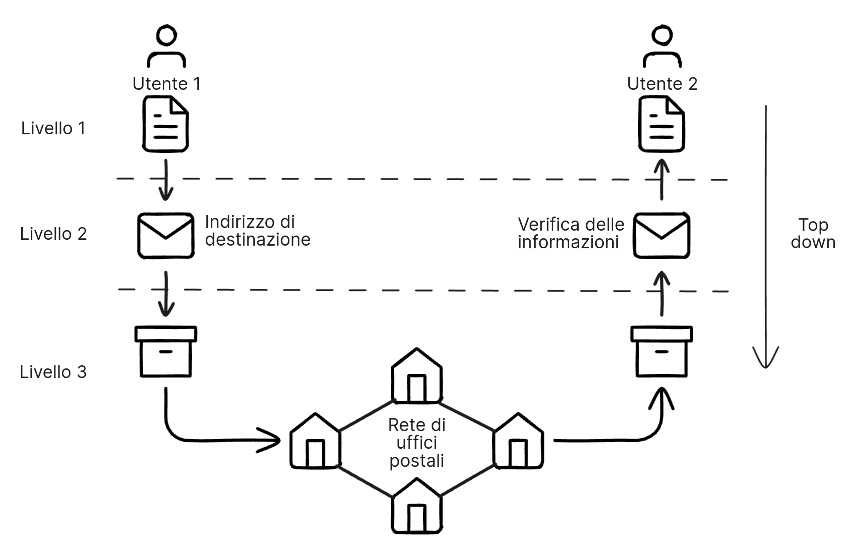
\includegraphics[width=0.95\textwidth]{rete-postale}
      \caption{Esempio di comunicazione tra 2 utenti}
    \end{figure}

    Il \textbf{Protocollo} è il linguaggio utilizzato per comunicare tra i 2
    utenti, mentre l'\textbf{Architettura di rete} è tutta quella infrastruttura
    che trasporta il messaggio tra i 2 utenti.
  \end{example}
\end{figure}

\noindent
La rappresentazione dei sistemi di comunicazione di solito viene fatta nella modalità
\textbf{top-down}, cioè si parte dal livello applicativo, quello più alto, fino a scendere
nei livelli più bassi in cui si trova la vera e propria architettura della rete.

\section{Architetture di rete}
Di solito si fa riferimento all'architettura più utilizzata, cioè la rete
\textbf{Internet}. Si possono distinguere i seguenti elementi base:
\begin{itemize}
  \item \textbf{Calcolatori (End host)}
  \item \textbf{Router (Intermediate host)}
  \item \textbf{Collegamenti}
\end{itemize}

\subsection{Reti locali}
Le reti locali, o \textbf{LAN} (Local Area Network), sono caratterizzate da un
\textbf{router di bordo} a cui sono collegati gli end host tramite \textbf{cavi fisici}
o collegamenti wireless.
\begin{figure}[H]
  \centering
  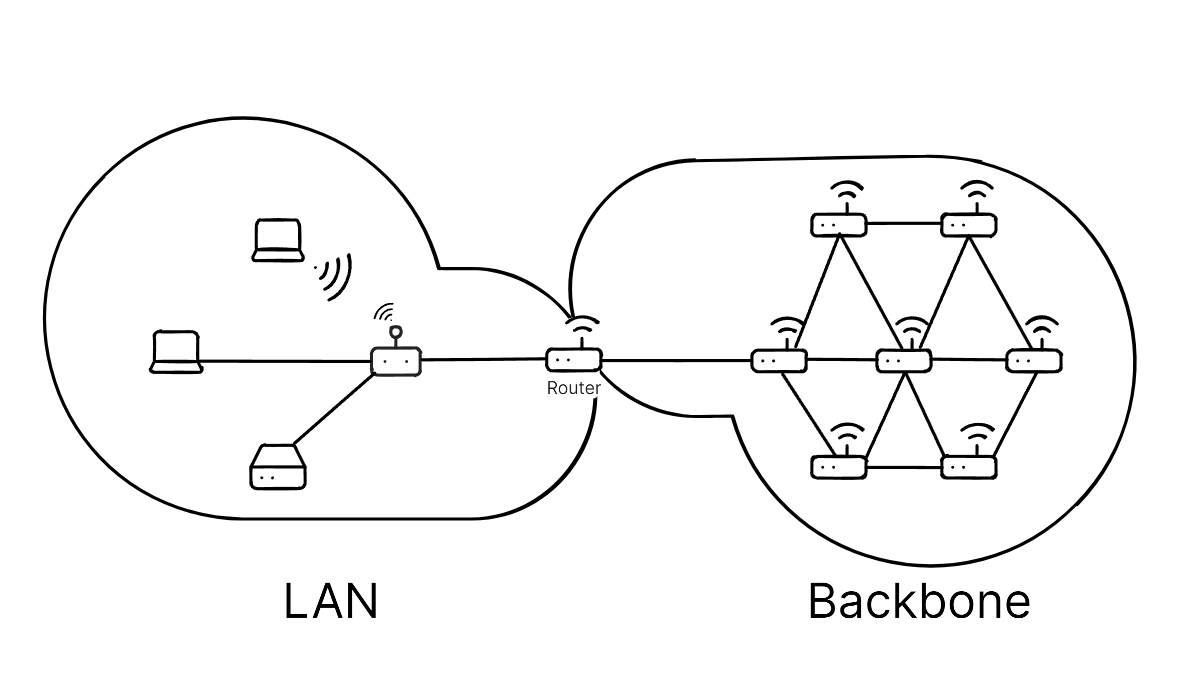
\includegraphics[width=0.95\textwidth]{lan-backbone}
  \caption{Rete locale}
\end{figure}

\vspace{1em}
\noindent
Per collegare diverse LAN tra loro esiste la \textbf{backbone}, cioè è una rete
di router collegati tra di loro con una topologia
gestita dal gestore della rete. Questi router sono geograficamente distribuiti
su tutto il territorio.
\begin{figure}[H]
  \centering
  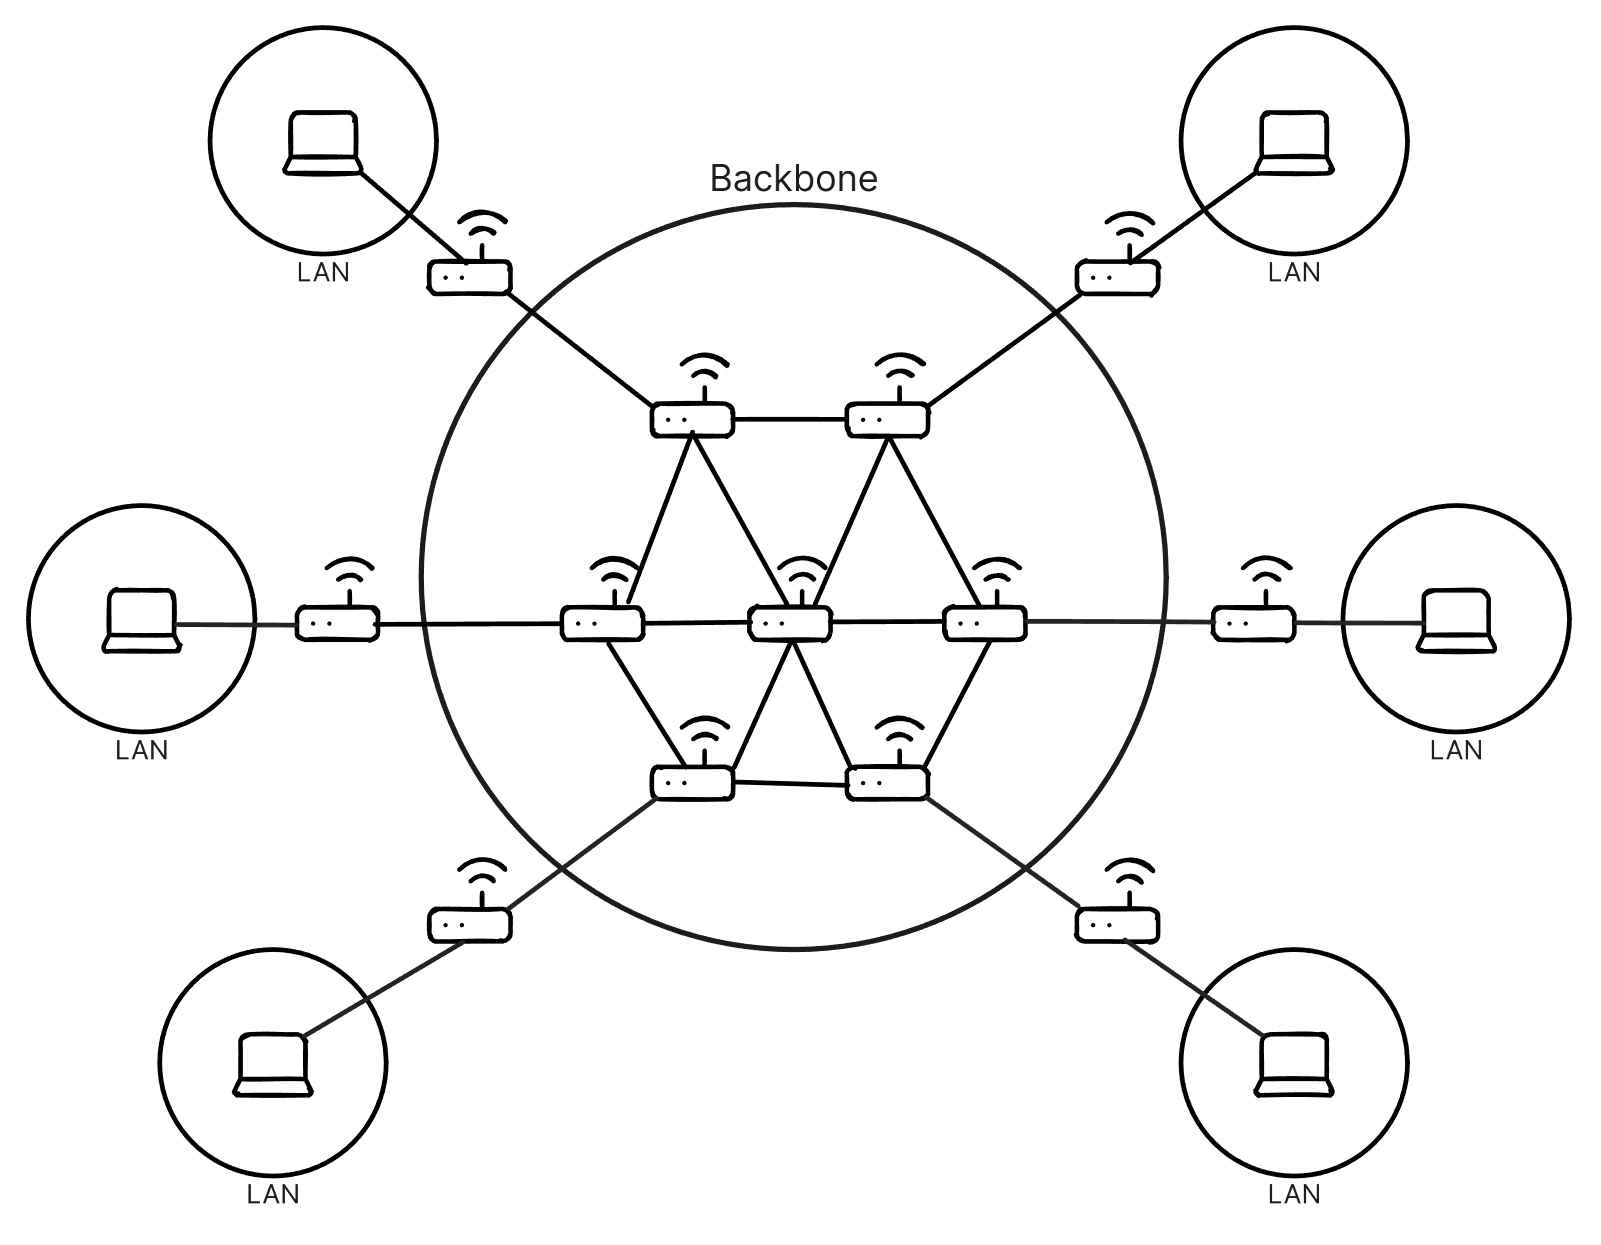
\includegraphics[width=0.95\textwidth]{internet}
  \caption{Intercollegamento di LAN}
\end{figure}

\noindent
Nella maggior parte delle volte le connessioni tra i router all'interno della
backbone sono cablate, di solito tramite fibre ottiche, soltanto in rari casi
si usano connessioni wireless.

\subsubsection{Organizzazione del Backbone}
Il backbone è composto da diverse reti che appartengono a diverse organizzazioni
permettendo di creare diverse interconnessioni tra le reti. Queste organizzazioni
si chiamano \textbf{Internet Service Provider} (ISP). Gli ISP hanno diversi livelli:
\begin{enumerate}
  \item \textbf{Livello 1}: Hanno una connessione internazionale
    e quindi sono in grado di comunicare con tutti gli altri ISP.
  \item \textbf{Livello 2}: Lavorano a livello nazionale.
  \item \textbf{Livello 3}: Lavorano a livello locale.
\end{enumerate}

\noindent
Gli ISP di livello 1 sono collegati tra di loro per permettere la comunicazione
tra ISP di livello 1 diversi. Anche gli ISP di livello più basso permettono
la comunicazione tra di loro o tra gli ISP di livello superiore, tutto questo
grazie ad accordi commerciali tra le varie organizzazioni.
\begin{figure}[H]
  \centering
  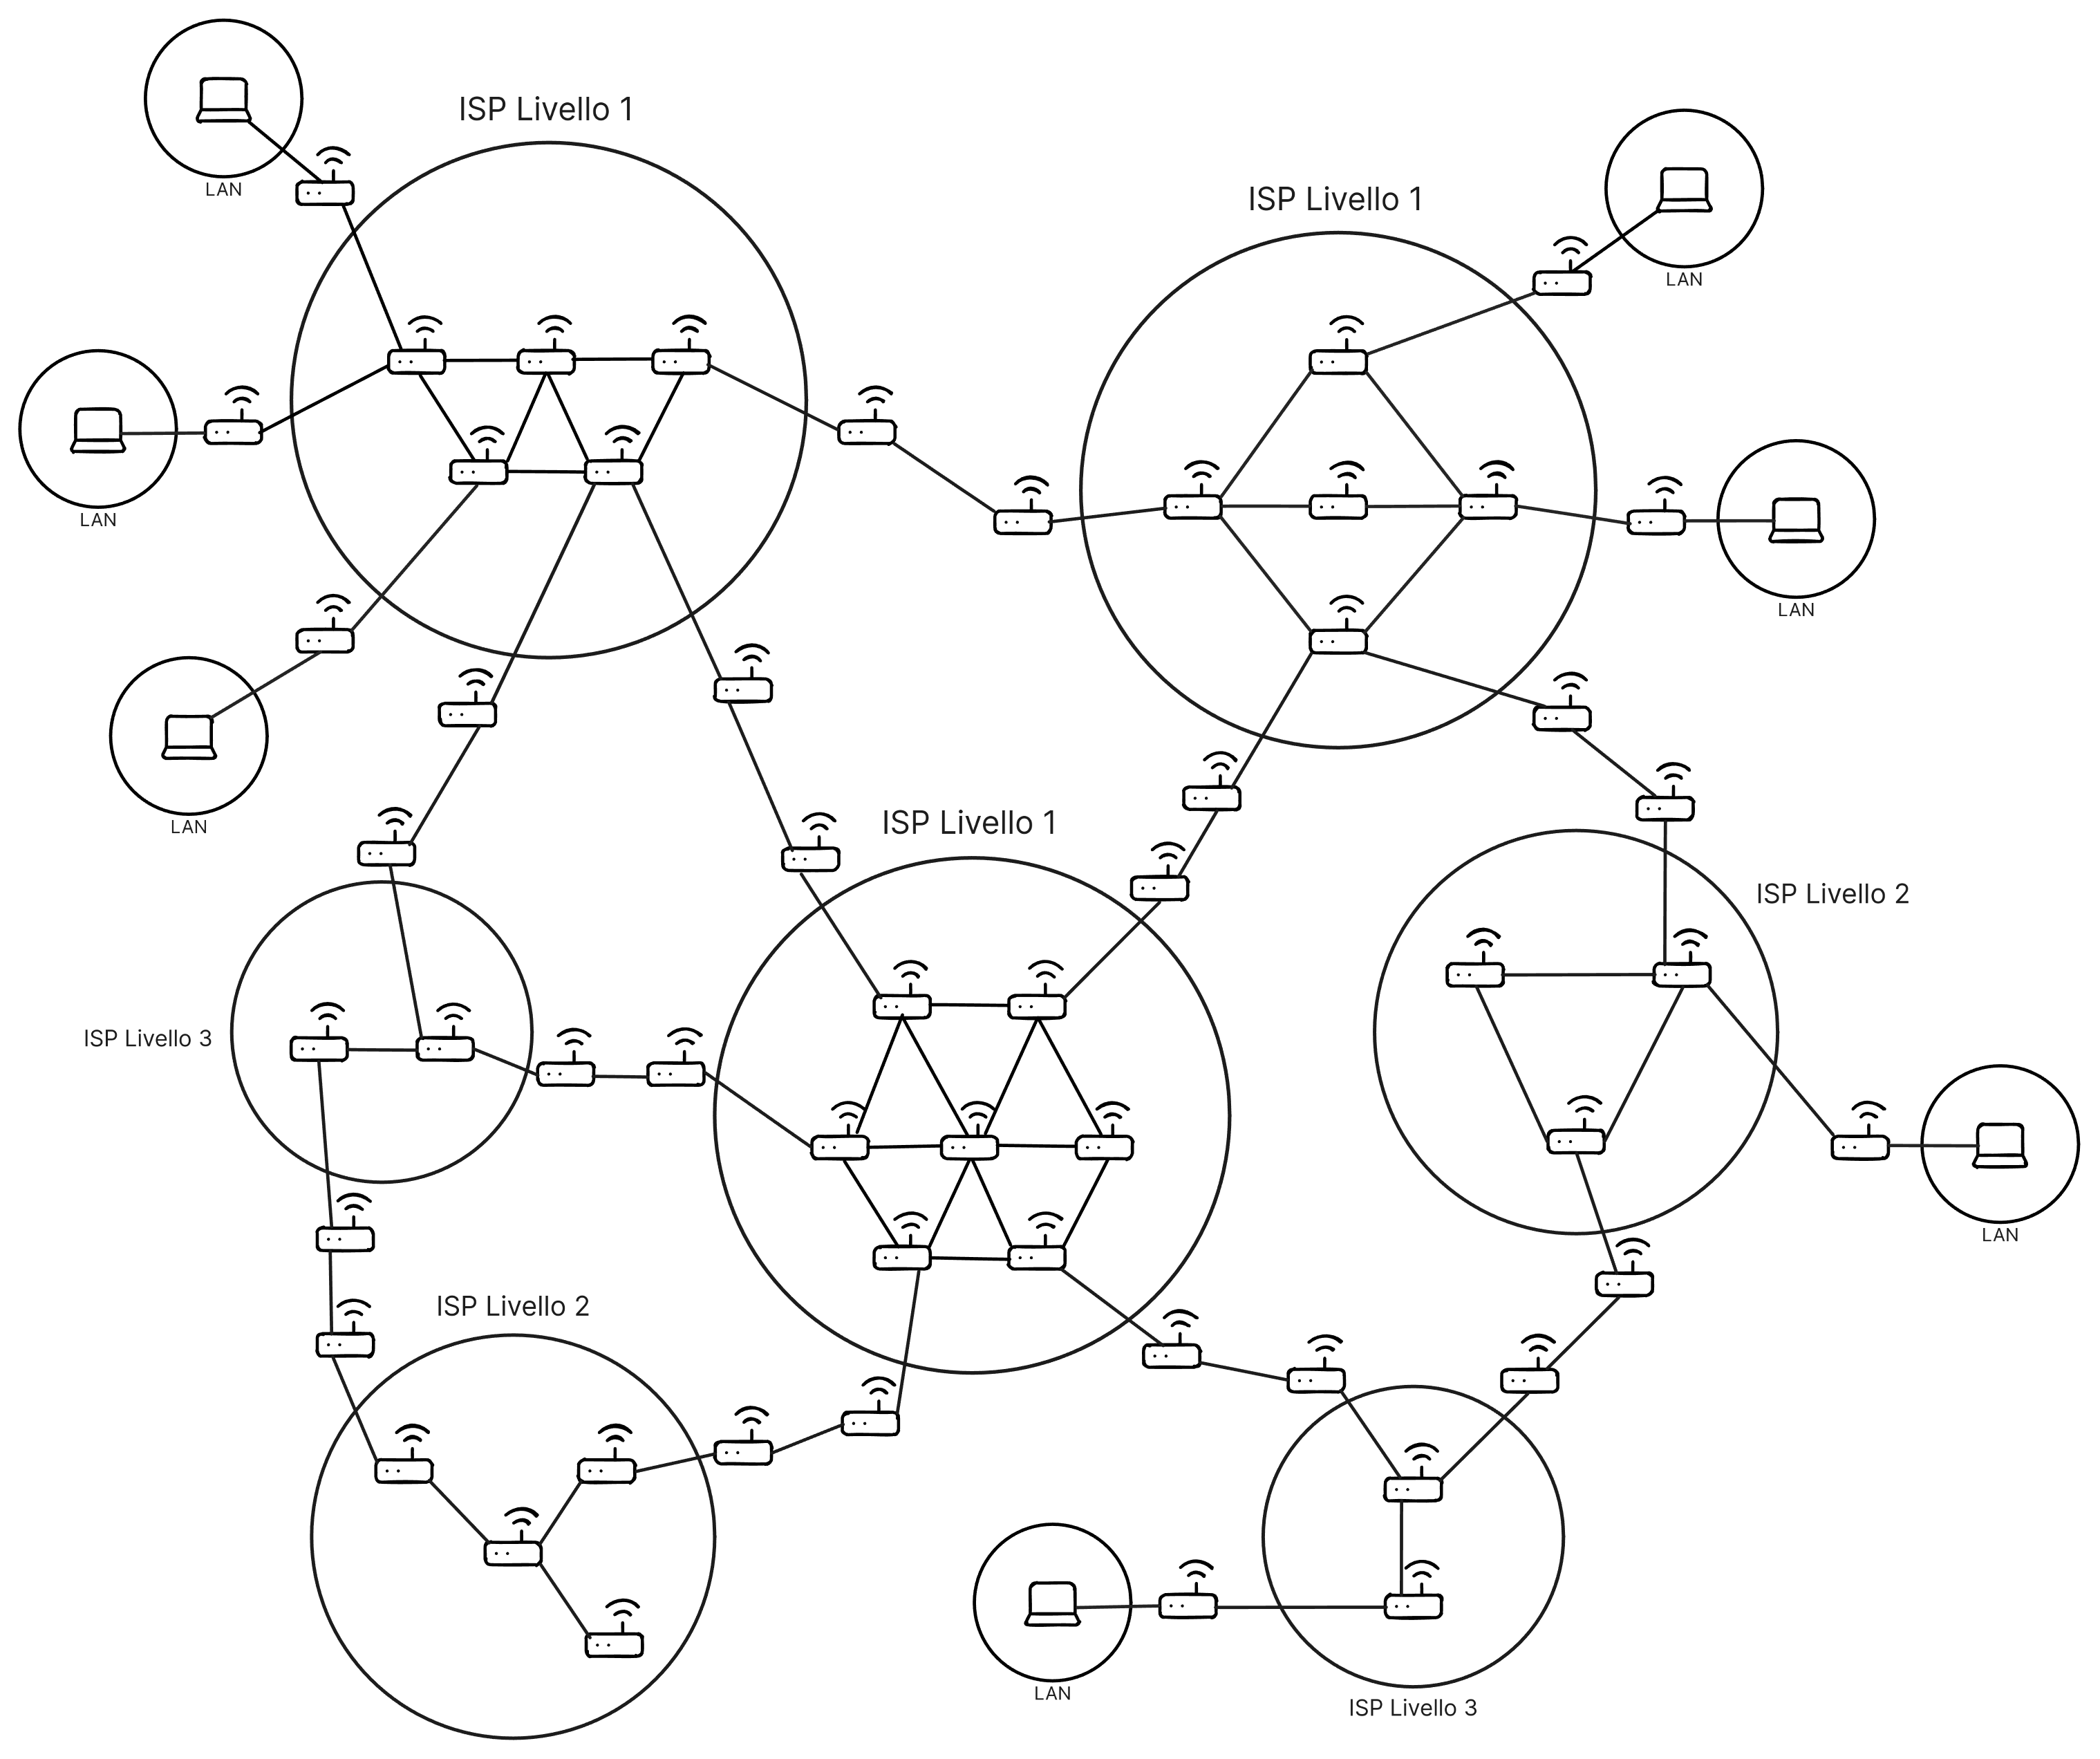
\includegraphics[width=0.95\textwidth]{livelli-di-isp}
  \caption{Livelli di ISP}
\end{figure}

\noindent
\textbf{Internet} è la \textbf{Rete delle reti}, cioè è la rete che collega
tutti gli ISP tra di loro ed è un organizzazione gerarchica, cioè è sufficiente
creare collegamenti con un sottoinsieme di ISP operanti sul territorio per permettere
il collegamento a tutta la rete.

\noindent
Di conseguenza, per raggiungere un utente, in genere, si segue un percorso gerarchico.
Un esempio è la rete stradale, dove per raggiungere una città si seguono le strade
principali e poi si scende in quelle secondarie.

\noindent
La scelta del percorso segue criteri basati su distanza e tempo.

\section{Modalità di comunicazione}
La gestione del trasporto dei messaggi è gestita dalla rete, però con che modalità
trasferisco l'informazione tra 2 utenti?

\subsection{Reti a commutazione di circuito}
È la modalità di commutazione che è stata utilizzata per la prima volta.

\noindent
In questa modalità le risorse (capacità del canale di trasmissione) vengono riservate \textbf{end-to-end}
per la comunicazione, cioè viene letteralmente riservato un circuito che viene
utilizzato dai 2 utenti.
\begin{figure}[H]
  \centering
  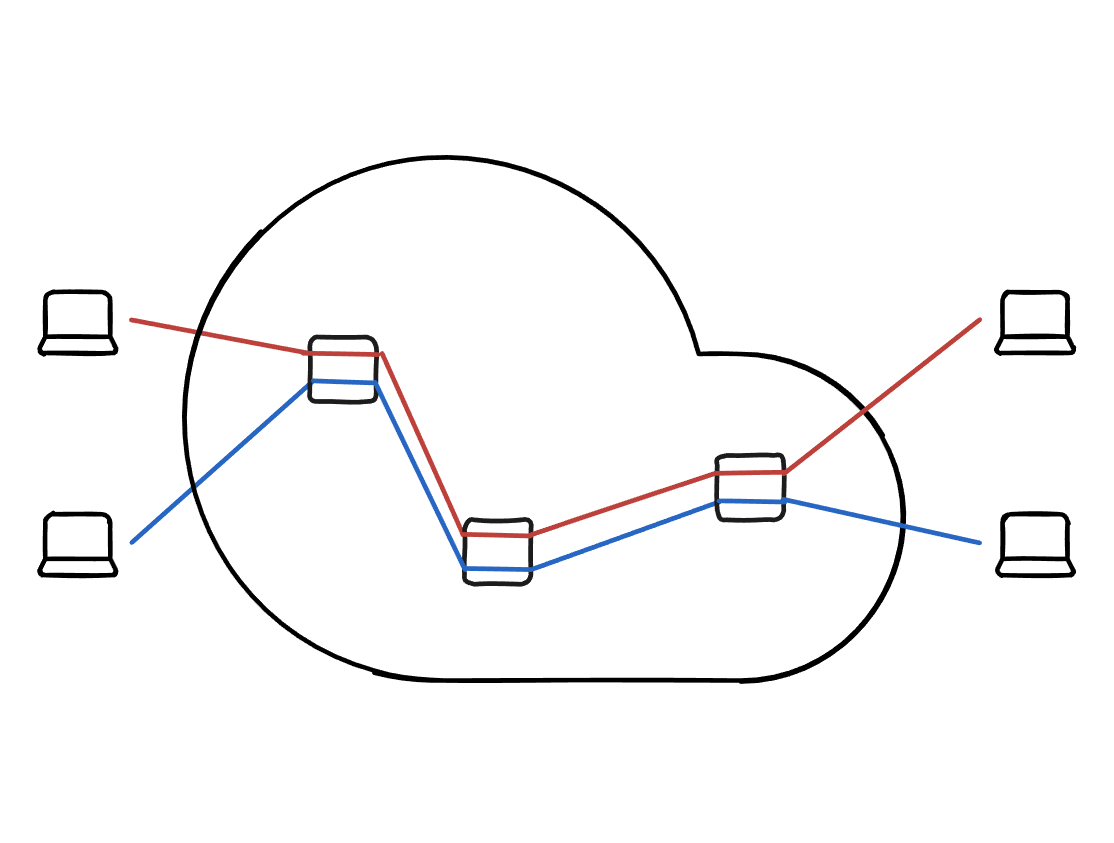
\includegraphics[width=0.95\textwidth]{comm-circuito}
  \caption{Commutazione di circuito}
\end{figure}

\noindent
Ogni canale è completamente dedicato alla comunicazione tra i 2 utenti, quindi
se più utenti vogliono comunicare tra di loro, bisogna riservare altre risorse.

\subsubsection{Vantaggi}
\begin{itemize}
  \item Risorse dedicate
  \item Ritardo deterministico

    \noindent
    \begin{itemize}
      \begin{figure}[H]
        \centering
        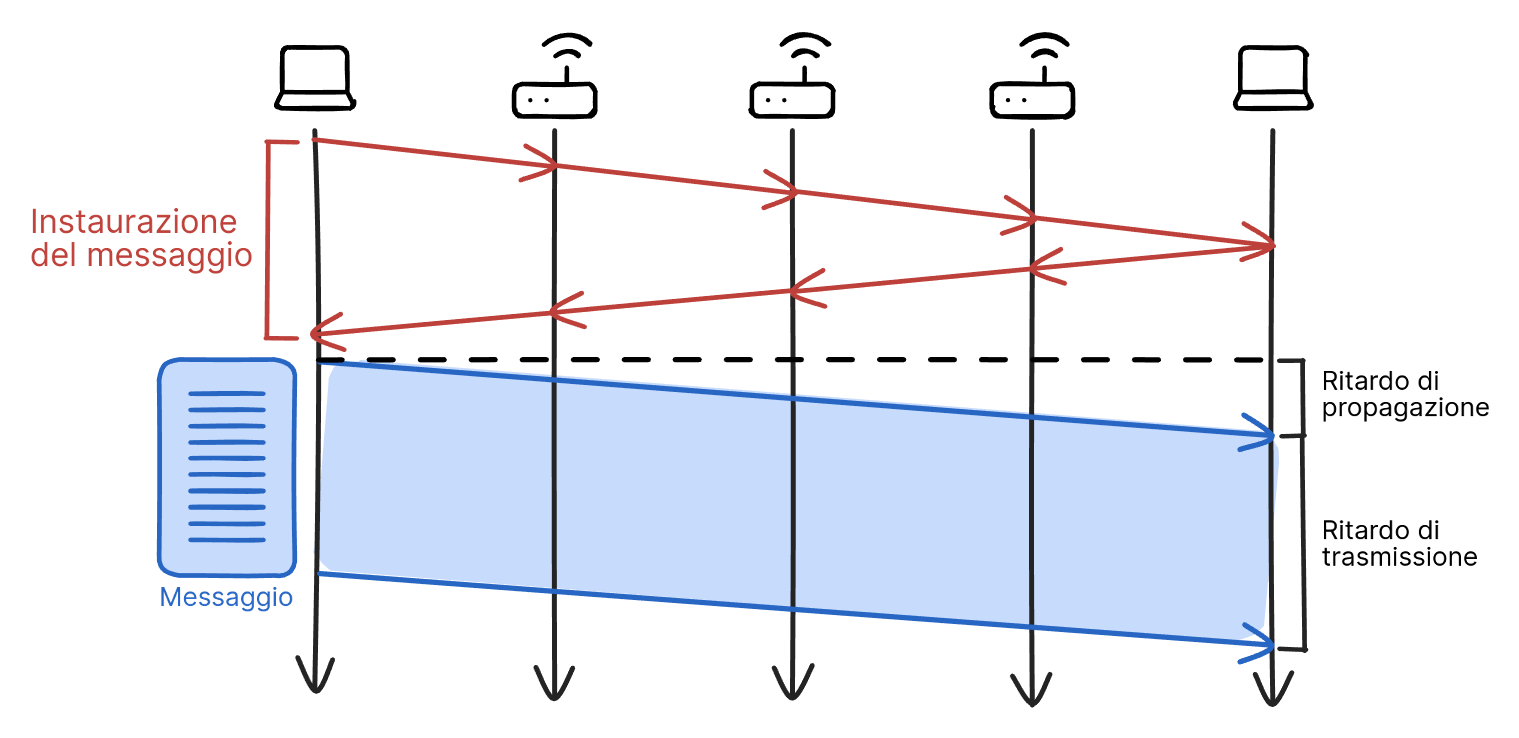
\includegraphics[width=0.95\textwidth]{ritardo}
        \caption{Ritardo}
      \end{figure}
      \item \textbf{Ritardo di trasmissione}: Tempo necessario per trasmettere il messaggio
      \item \textbf{Ritardo di propagazione}: Tempo necessario per trasmettere il messaggio
        da un nodo all'altro
    \end{itemize}
    Se il messaggio è grande \( L\,bit \) e il canale riservato è di \( B\,bit/s \),
    allora il tempo di trasmissione sarà:
    \[
    T = \frac{L}{B}
    \] 
    Il ritardo di trasmissione e di propagazione è deterministico, perchè
    dato il circuito di trasmissione, il tempo di trasmissione è noto.
\end{itemize}

\subsubsection{Svantaggi}
Nel corso di utilizzo sporadico si ha uno spreco di risorse, perchè il circuito
viene riservato per tutta la durata della comunicazione, anche se i 2 utenti
non stanno comunicando.
\begin{figure}[H]
  \centering
  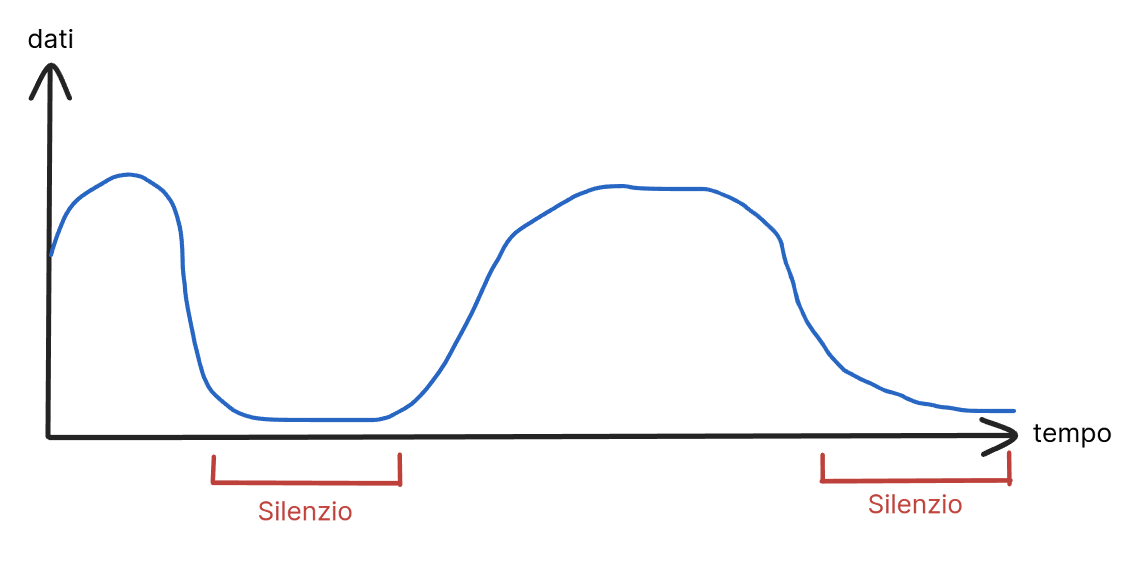
\includegraphics[width=0.70\textwidth]{silenzio}
  \caption{Spreco di risorse}
\end{figure}

\subsection{Reti a commutazione di pacchetto}
È la modalità di commutazione più utilizzata al giorno d'oggi.

\noindent
L'informazione (messaggio) viene suddivisa in \textbf{pacchetti} e ad ogni
pacchetto viene aggiunto un \textbf{header} per permettere:
\begin{itemize}
  \item La consegna del pacchetto stesso
  \item La ricostruzione del messaggio
\end{itemize}

Il messaggio è l'informazione da trasferire, mentre il pacchetto è una porzione
del messaggio stesso.

\noindent
Il messaggio prima della trasmissione viene separato in unità più piccole e a
queste unità viene aggiunta un'intestazione che serve a rendere le unità indipendenti
per poterle trasmettere in modo indipendente. L'intestazione permette la consegna del
pacchetto perchè contiene la destinazione del pacchetto e la ricostruzione del messaggio
perchè contiene il numero di sequenza del pacchetto.
\begin{figure}[H]
  \centering
  \begin{tikzpicture}
    \node[draw, minimum width=5cm, minimum height=1cm] at (0.45,0) (m) {Messaggio};
    \draw[->] (m.south) -- ++(0,-1);

    \coordinate (a) at (-2.7,-3);
    \draw (a) rectangle ++(1,1) node[midway] {$m_1$};
    \draw[blue,fill, fill opacity=0.1] (a) ++(0,1) rectangle ++(-0.5,-1);

    \coordinate (b) at (-0.8,-3);
    \draw (b) rectangle ++(1,1) node[midway] {$m_2$};
    \draw[blue,fill, fill opacity=0.1] (b) ++(0,1) rectangle ++(-0.5,-1);

    \coordinate (c) at (1.1,-3);
    \draw (c) rectangle ++(1,1) node[midway] {$m_3$};
    \draw[blue,fill, fill opacity=0.1] (c) ++(0,1) rectangle ++(-0.5,-1);

    \coordinate (d) at (2.9,-3);
    \draw (d) rectangle ++(1,1) node[midway] {$m_4$};
    \draw[blue,fill, fill opacity=0.1] (d) ++(0,1) rectangle ++(-0.5,-1);
    \draw[<-,blue] (d) ++(-0.25,1) -- ++(0,0.5) node[above,blue] {Header};

  \end{tikzpicture}
  \caption{Messaggio e pacchetti}
\end{figure}

\noindent I pacchetti vengono salvati all'interno di un \textbf{buffer}, cioè una
memoria temporanea, in attesa di essere trasmessi. Man mano che i pacchetti
vengono inviati vengono accumulati nel buffer dei router e questo avviene per
qualsiasi collegamento.
\begin{figure}[H]
  \centering
  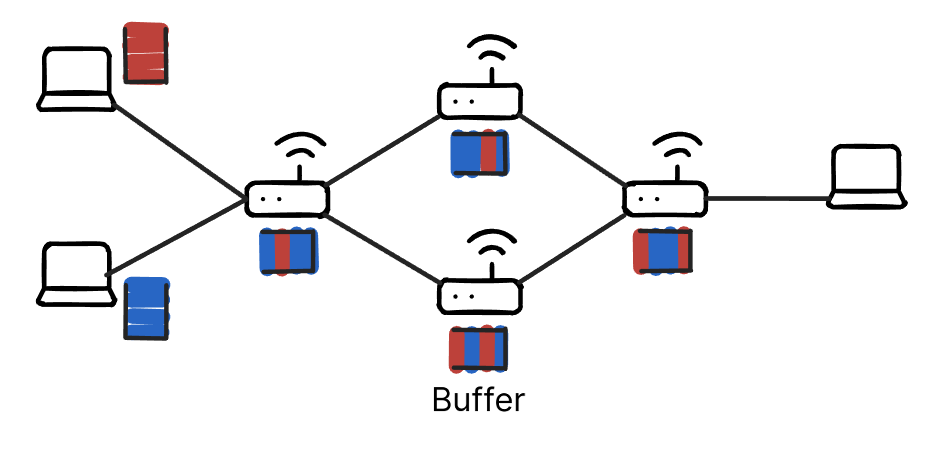
\includegraphics[width=0.95\textwidth]{buffer}
  \caption{Rappresentazione del buffer}
\end{figure}

\noindent
I pacchetti possono arrivare in ordine diverso rispetto a quello di trasmissione,
però grazie all'header è possibile ricostruire il messaggio originale.

\subsubsection{Vantaggi}
\begin{itemize}
  \item Utilizza le risorse solo quando ci sono pacchetti da trasmettere e questo
    viene chiamato \textbf{commutazione statistica}.
  \item \textbf{Multiplazione statistica}, cioè utilizzo lo stesso
    canale per trasmettere più pacchetti di utenti diversi.
\end{itemize}

\subsubsection{Svantaggi}
\begin{itemize}
  \item Potenziale perdita dei pacchetti: La memoria dei buffer ha una capacità finita,
    quindi se il tasso di ricezione dei pacchetti è superiore al tasso di
    smaltimento del buffer, esso inizia a riempirsi. Le perdite aumentano la
    complessità di gestione della rete.

  \item Ritardi aumentati

    \noindent
    I router prima di trasmettere i pacchetti, deve aspettare di ricevere tutti
    i pacchetti. Questo si chiama \textbf{store \& forward}. Di conseguenza
    più aumentano i router, più aumenta il ritardo di trasmissione.
    \begin{figure}[H]
      \centering
      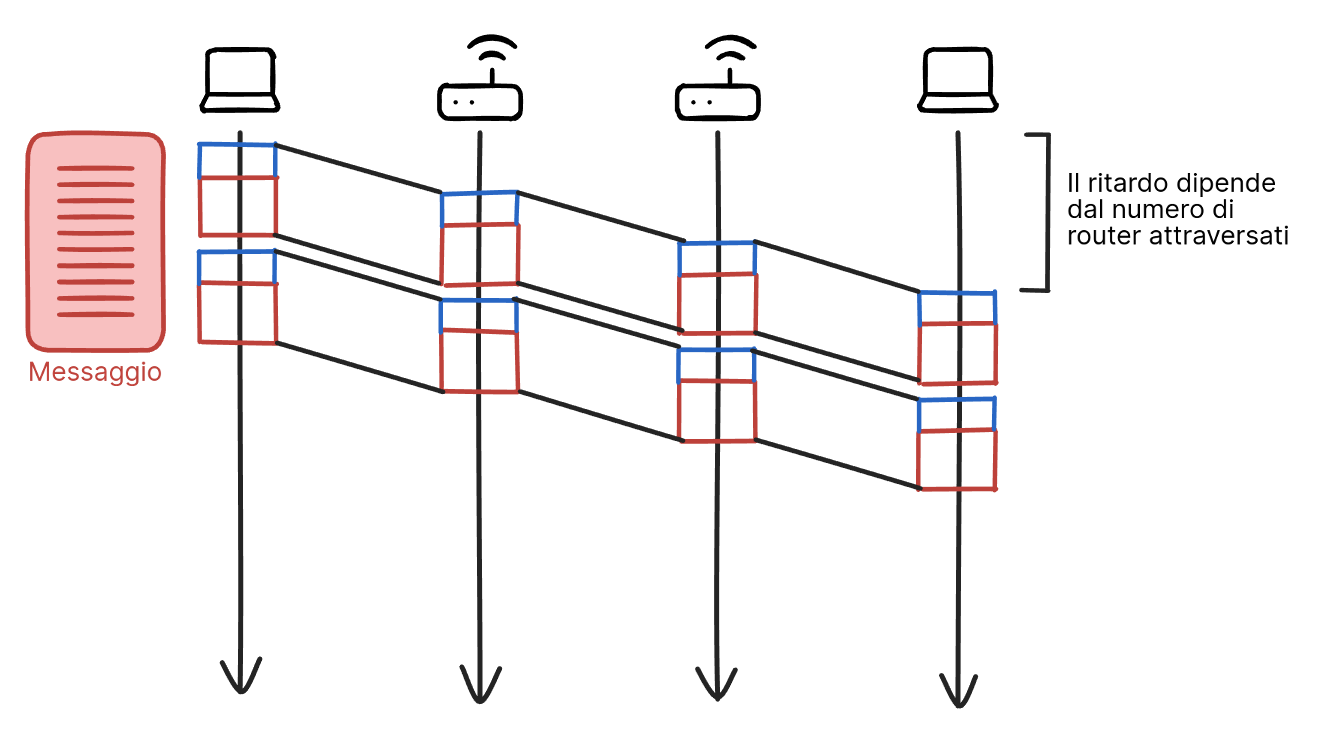
\includegraphics[width=0.95\textwidth]{ritardo-pacchetti}
      \caption{Ritardo di trasmissione dei pacchetti}
    \end{figure}
\end{itemize}

\section{Ritardi di trasmissione}
\begin{figure}[H]
  \centering
  \begin{tikzpicture}
    \draw (0,0) rectangle ++(3,3);
    \node[above] at (1.5,3) {Router};

    % Buffers
    \draw (2.3,2.8) -- ++(0.5,0) -- ++(0,-0.4) -- ++(-0.5,0) node[above left, scale=0.8]
      {Buffer};
    \draw (2.3,2.2) -- ++(0.5,0) -- ++(0,-0.4) -- ++(-0.5,0);
    \node at (2.6,1.6) {$\vdots$};
    \draw (2.3,1.17) -- ++(0.5,0) -- ++(0,-0.4) -- ++(-0.5,0);
    \draw (2.3,0.57) -- ++(0.5,0) -- ++(0,-0.4) -- ++(-0.5,0);

    % Inputs
    \draw (0,2.6) -- ++(-0.5,0);
    \draw (0,2.0) -- ++(-0.5,0);
    \node at (-0.25,1.6) {$\vdots$};
    \draw (0,1.0) -- ++(-0.5,0);
    \draw (0,0.4) -- ++(-0.5,0);

    \draw (-0.8,2.8) -- ++(-0.3,0) -- ++(0,-2.6) node[midway,left,align=center]
      {n° ingressi} -- ++(0.3,0);

    % Outputs
    \draw (3,2.6) -- ++(0.5,0);
    \draw (3,2.0) -- ++(0.5,0);
    \node at (3.25,1.6) {$\vdots$};
    \draw (3,1.0) -- ++(0.5,0);
    \draw (3,0.4) -- ++(0.5,0);

    \draw (3.8,2.8) -- ++(0.3,0) -- ++(0,-2.6) node[midway,right,align=center]
      {n° uscite} -- ++(-0.3,0);
  \end{tikzpicture}
  \caption{Struttura di un router}
\end{figure}

Su un singolo router le componenti principali del ritardo sono:
\begin{itemize}
  \item \textbf{Ritardo di elaborazione al nodo}: Tempo necessario per elaborare
    il pacchetto.
  \item \textbf{Ritardo di accodamento}: È il tempo speso nel buffer prima che
    il pacchetto venga trasmesso ed è la componente principale tra tutti i
    ritardi. (\( \frac{L}{B} \))
  \item \textbf{Ritardo di trasmissione}: Tempo necessario per trasmettere il
    pacchetto.
  \item \textbf{Ritardo di propagazione}: Tempo necessario per trasmettere il
    pacchetto da un nodo all'altro.
\end{itemize}

\subsection{Ordine di grandezza}
Dipende dalla distanza e dalla velocità di trasmissione del collegamento. La
distanza si distingue in:
\begin{itemize}
  \item \textbf{Locale}: \( < 10ms \) 
  \item \textbf{Internazionale}: \( 20-40ms \) 
  \item \textbf{Intercontinentale}: \( > 100ms \)
\end{itemize}

\subsection{Strumenti per calcolare il ritardo end-to-end}
\subsubsection{Ping}
Dati 2 utenti in 2 LAN diverse, il ping manda un pacchetto all'utente di destinazione
e l'utente che lo ha mandato prima o poi riceverà un messaggio di risposta (\textbf{
echo reply}). Il tempo che passa tra l'invio del pacchetto e la ricezione del
messaggio di risposta è il ritardo end-to-end.

\vspace{1em}
\noindent
Non si può sapere se il ritardo è asimmetrico o no, cioè se il ritardo di andata è uguale
al ritardo di ritorno, ma si può soltanto calcolare il ritardo totale.
\begin{figure}[H]
  \centering
  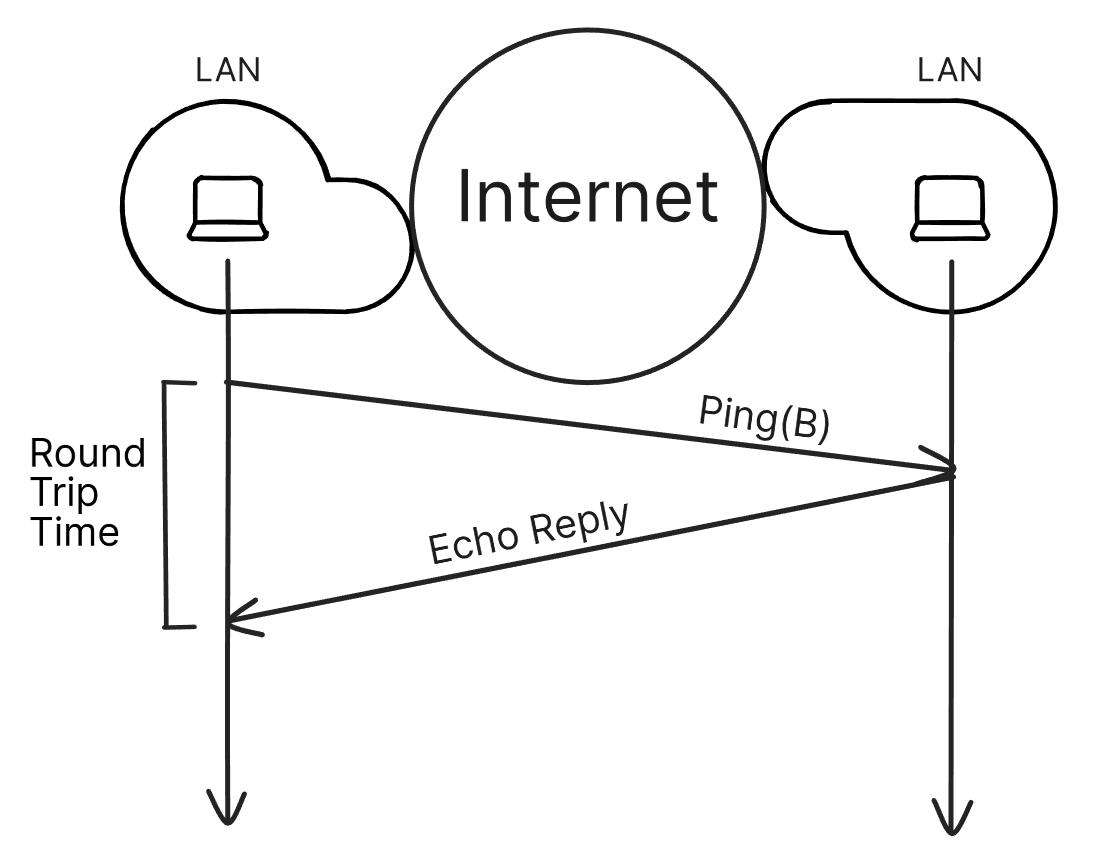
\includegraphics[width=0.70\textwidth]{ping}
  \caption{Ping}
\end{figure}

\noindent
Se si esegue il comando \texttt{ping} da un terminale si riceve il seguente output:
\begin{figure}[H]
  \centering
  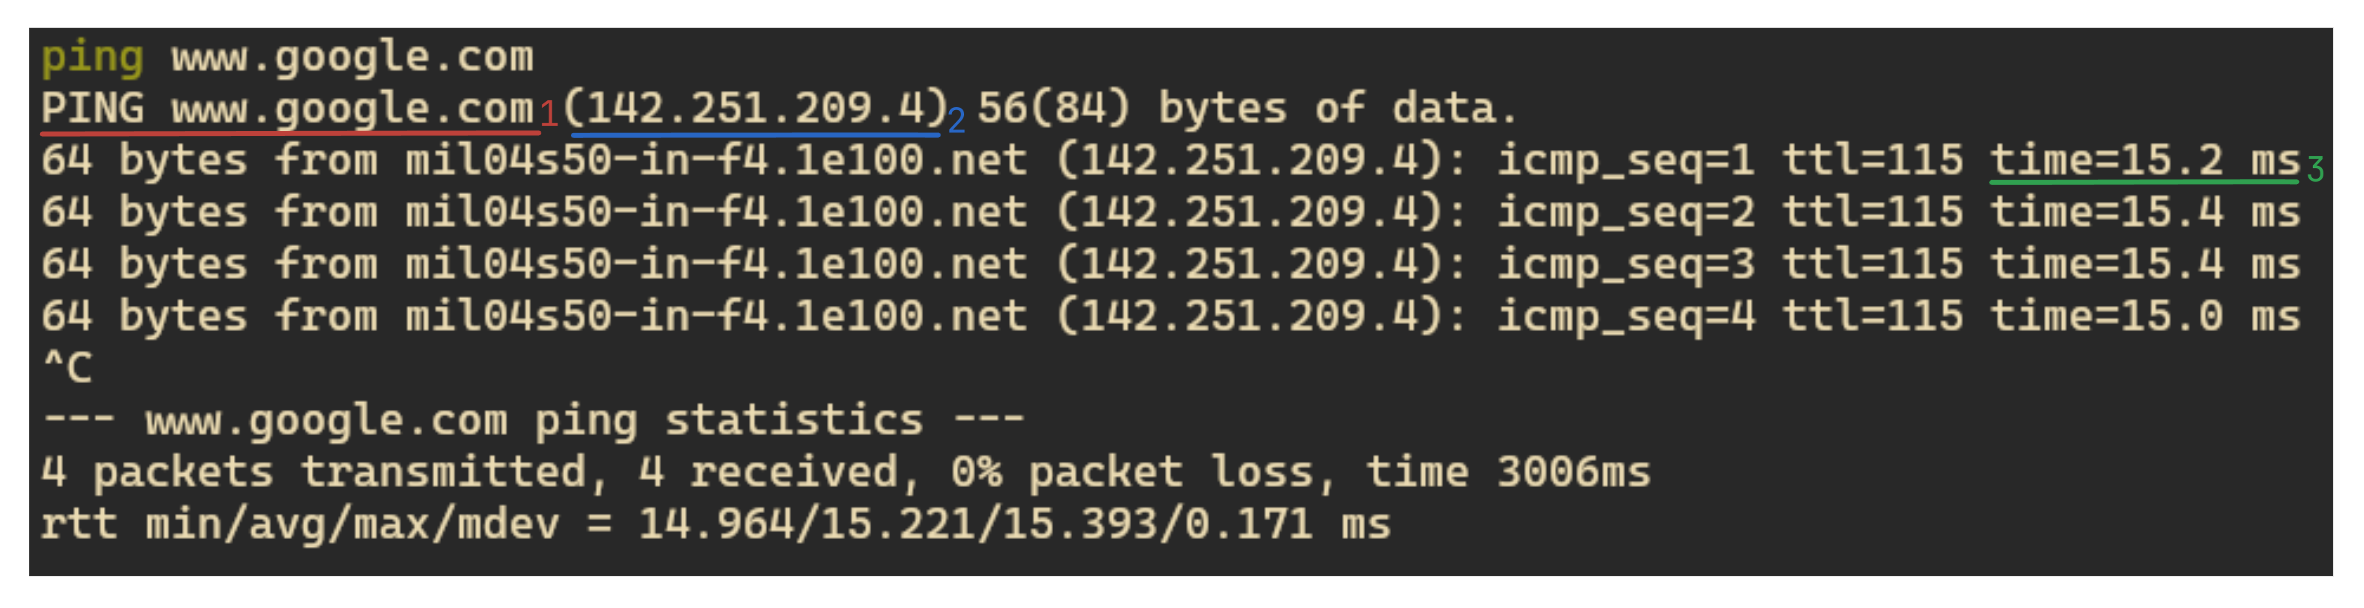
\includegraphics[width=1\textwidth]{ping-cmd}
  \caption{Output di ping}
\end{figure}

\begin{enumerate}
  \item Viene rieseguito il ping facendo riferimento al \textbf{server fisico}
  \item Tra parentesi viene rappresentato l'indirizzo che identifica il server, chiamato
    \textbf{indirizzo IP}
  \item Alla fine c'è il tempo di risposta del server
\end{enumerate}

\subsubsection{Traceroute}
Vengono mandati 3 messaggi al primo router e si calcolano i tempi di risposta tra
il primo utente e il primo router, poi viene fatta la stessa cosa con i seguenti
router fino ad arrivare all'utente di destinazione.
\begin{figure}[H]
  \centering
  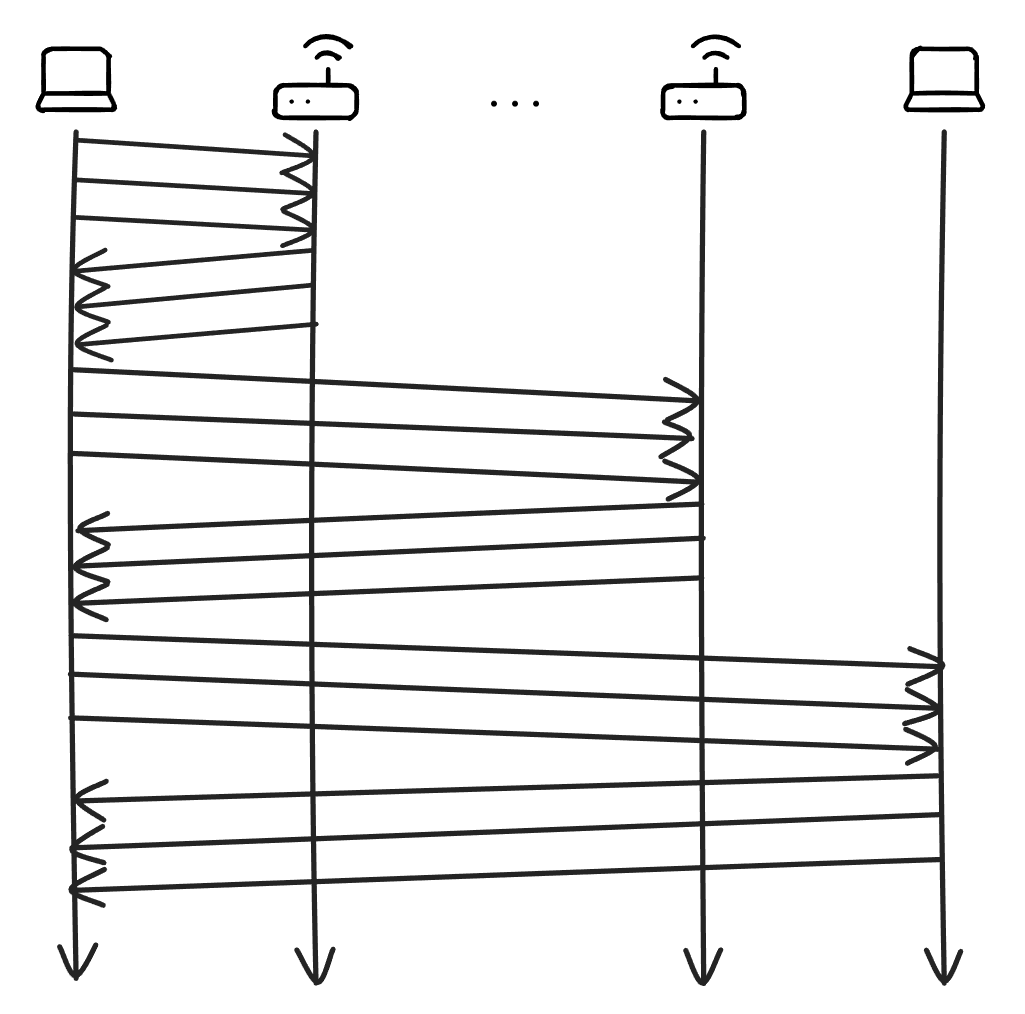
\includegraphics[width=0.70\textwidth]{traceroute}
  \caption{Traceroute}
\end{figure}

\noindent
Se si esegue il comando \texttt{traceroute} da un terminale si riceve il seguente output:
\begin{figure}[H]
  \centering
  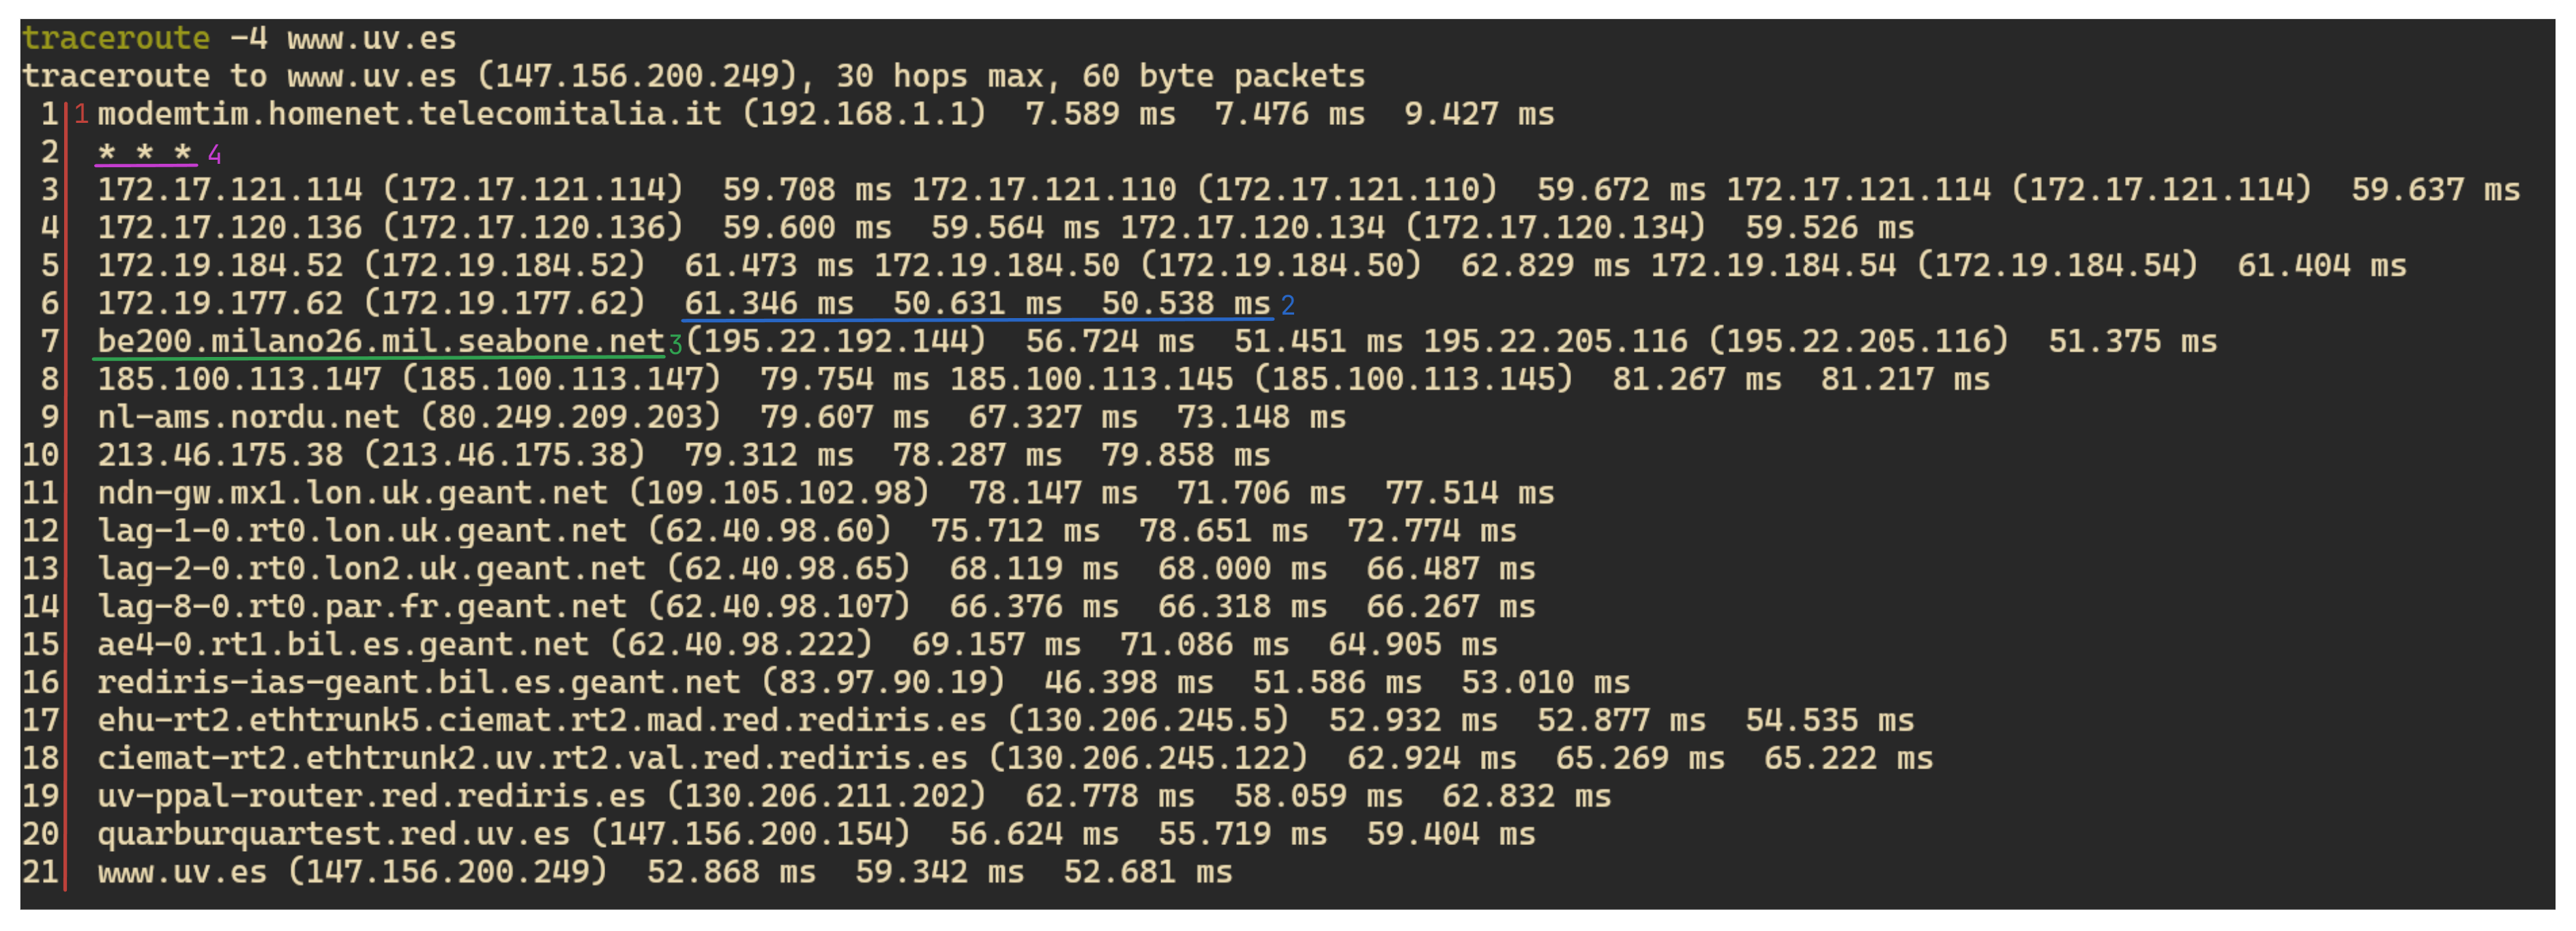
\includegraphics[width=1\textwidth]{traceroute-cmd}
  \caption{Output di traceroute}
\end{figure}

\begin{enumerate}
  \item Indica il numero di router attraversati
  \item Stampa i valori di ritardo dei 3 pacchetti trasmessi
  \item È il nome logico del router che si sta attraversando, da questo nome si può
    dedurre la posizione geografica del router e l'ISP a cui appartiene
  \item Gli asterischi indicano che il router è stato configurato in modo da ignorare
    i pacchetti e non mandare alcuna risposta, questo perchè serve soltanto a inoltrare
    i pacchetti ad un altro router.
\end{enumerate}


\subsection{Quantità di dati trasferiti}
La quantità di informazioni che si riesce a trasmettere si misura in \( \frac{bit}{s} \)
e questa informazione dipende dalla capacità di tutti i canali di trasmissione
attraversati.

\noindent
Ogni canale avrà una dimensione diversa e si può determinare la banda totale a
disposizione (\textbf{Throughput}) dal \textbf{collo di bottiglia}, cioè dalla minore
capacità di trasmissione tra tutti i canali attraversati.
\begin{figure}[H]
  \centering
  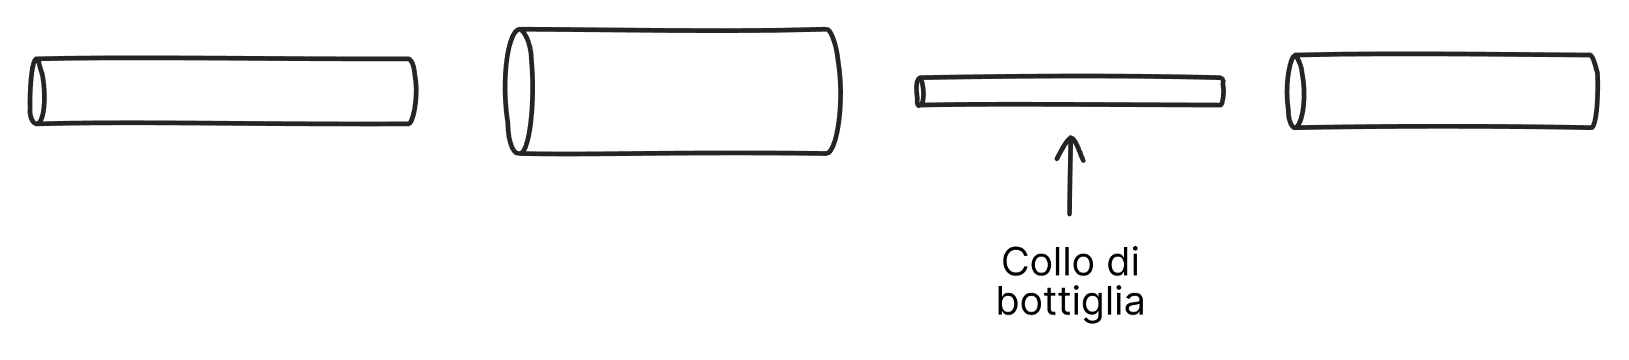
\includegraphics[width=0.70\textwidth]{throughput}
  \caption{Throughput}
\end{figure}

\section{Modello a strati}
Il modello a strati affronta la \textbf{comunicazione tra due entità} secondo la modalità
\textbf{divide et impera}.
\begin{figure}[H]
  \centering
  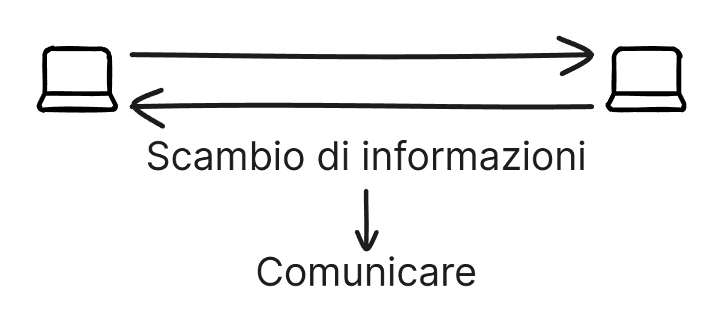
\includegraphics[width=0.70\textwidth]{comunicazione}
\end{figure}
\noindent
Per scambiare informazioni le due entità devono comunicare. La comunicazione si divide in:
\begin{itemize}
  \item \textbf{Comunicazione logica}: Gestisce le problematiche relative all'informazione

    \noindent Ad esempio:
    \begin{itemize}
      \item Linguaggio utilizzato
      \item Come comportarsi nello scambio
    \end{itemize}

  \item \textbf{Comunicazione Fisica}: Come trasferire i diversi bit. Il contenuto
    dell'informazione non è importante.
\end{itemize}

\begin{figure}[H]
  \centering
  \begin{tikzpicture}
    \draw (0,0) rectangle ++(3,-1) node[midway,draw] {Messaggio};
    \node[left,align=right,scale=0.7] at (0,-0.5)
      {Livello/Strato};

    \draw (0,-1) rectangle ++(3,-1);
    \node[blue,left,align=right,scale=0.7] at (0,-1.5)
      {Header specifico al livello\\Es: n° di sequenza};

    \draw (0,-2) rectangle ++(3,-1);
    \node[red,left,align=right,scale=0.7] at (0,-2.5)
      {Header specifico al livello\\Es: Indirizzo di destinazione};

    \draw (0,-3) rectangle ++(3,-1) node[midway] {$1101010010101001$};

    \coordinate (r1) at (0.4,-1.75);
    \draw[red] (r1) rectangle ++(0,0.5);
    \draw[blue] (r1) ++(0,0.5) rectangle ++(0.25,-0.5);
    \draw (r1) ++(0,0.5) ++(0.25,-0.5) rectangle ++(0.5,0.5) node[below right,yshift=-0.1cm] {$\ldots$};

    \coordinate[right of=r1, xshift=0.4cm] (r2);
    \draw[red] (r2) rectangle ++(0,0.5);
    \draw[blue] (r2) ++(0,0.5) rectangle ++(0.25,-0.5);
    \draw (r2) ++(0,0.5) ++(0.25,-0.5) rectangle ++(0.5,0.5);


    \coordinate (r3) at (0.18,-2.75);
    \draw[red] (r3) rectangle ++(0.25,0.5);
    \draw[blue] (r3) ++(0.25,0.5) rectangle ++(0.25,-0.5);
    \draw (r3) ++(0.25,0.5) ++(0.25,-0.5) rectangle ++(0.5,0.5) node[below right,yshift=-0.1cm] {$\ldots$};

    \coordinate[right of=r3, xshift=0.65cm] (r4);
    \draw[red] (r4) rectangle ++(0.25,0.5);
    \draw[blue] (r4) ++(0.25,0.5) rectangle ++(0.25,-0.5);
    \draw (r4) ++(0.25,0.5) ++(0.25,-0.5) rectangle ++(0.5,0.5);

    \draw[->] (3.2,0) -- ++(0,-3);



    \draw (5,0) rectangle ++(3,-1) node[midway,draw] {Messaggio};
    \draw (5,-1) rectangle ++(3,-1);
    \draw (5,-2) rectangle ++(3,-1);

    \draw (5,-3) rectangle ++(3,-1) node[midway] {$1101010010101001$};

    \coordinate (r1) at (5.4,-1.75);
    \draw[red] (r1) rectangle ++(0,0.5);
    \draw[blue] (r1) ++(0,0.5) rectangle ++(0.25,-0.5);
    \draw (r1) ++(0,0.5) ++(0.25,-0.5) rectangle ++(0.5,0.5) 
      node[below right,yshift=-0.1cm] {$\ldots$};

    \coordinate[right of=r1, xshift=0.4cm] (r2);
    \draw[red] (r2) rectangle ++(0,0.5);
    \draw[blue] (r2) ++(0,0.5) rectangle ++(0.25,-0.5);
    \draw (r2) ++(0,0.5) ++(0.25,-0.5) rectangle ++(0.5,0.5);


    \coordinate (r3) at (5.18,-2.75);
    \draw[red] (r3) rectangle ++(0.25,0.5);
    \draw[blue] (r3) ++(0.25,0.5) rectangle ++(0.25,-0.5);
    \draw (r3) ++(0.25,0.5) ++(0.25,-0.5) rectangle ++(0.5,0.5) 
      node[below right,yshift=-0.1cm] {$\ldots$};

    \coordinate[right of=r3, xshift=0.65cm] (r4);
    \draw[red] (r4) rectangle ++(0.25,0.5);
    \draw[blue] (r4) ++(0.25,0.5) rectangle ++(0.25,-0.5);
    \draw (r4) ++(0.25,0.5) ++(0.25,-0.5) rectangle ++(0.5,0.5);

    \draw[<-] (4.8,0) -- ++(0,-3);

    \draw[->,dashed] (3,-3.5) -- ++(2,0) node[midway,below,align=center,scale=0.8] {Trasmissione\\fisica};
  \end{tikzpicture}
  \caption{Comunicazione tra due entità}
\end{figure}
\noindent
Ad ogni \textbf{livello} (o strato) viene elaborata parzialmente l'informazione e
trasformata. Ogni livello aggiunge un \textbf{header} che contiene un'informazione
specifica a quel livello, seguendo un \textbf{protocollo} (specifico per quel livello).

\vspace{1em}
\noindent
Ogni livello ha uno o più protocolli associati, e l'insieme dei protocolli di tutti i
livelli è chiamato \textbf{stack protocollare}.

\subsection{Stack ISO/OSI}
Il modello \textbf{ISO/OSI} (International Standard Organization / Open System Interconnection)
definisce dei livelli a seconda del sistema:
\begin{itemize}
  \item \textbf{End system}:
    \begin{figure}[H]
      \centering
      \begin{tikzpicture}[scale=0.8]
        \draw (0,6) rectangle ++(3,1) node[midway] {Applicazione};
        \draw (0,5) rectangle ++(3,1) node[midway] {Presentazione};
        \draw (0,4) rectangle ++(3,1) node[midway] {Sessione};
        \draw (0,3) rectangle ++(3,1) node[midway] {Trasporto};
        \draw (0,2) rectangle ++(3,1) node[midway] {Rete};
        \draw (0,1) rectangle ++(3,1) node[midway,align=center] {Collegamento\\dati};
        \draw (0,0) rectangle ++(3,1) node[midway] {Fisico};
        \node[below] at (1.5,0) {End system};
      \end{tikzpicture}
      \caption{Stack ISO/OSI per l'end system}
    \end{figure}
  \item \textbf{Intermediate system}:
    \begin{figure}[H]
      \centering
      \begin{tikzpicture}[scale=0.8]
        \draw (0,2) rectangle ++(3,1) node[midway] {Rete};
        \draw (0,1) rectangle ++(3,1) node[midway,align=center] {Collegamento\\dati};
        \draw (0,0) rectangle ++(3,1) node[midway] {Fisico};
        \node[below] at (1.5,0) {Intermediate system};
      \end{tikzpicture}
      \caption{Stack ISO/OSI per l'intermediate system}
    \end{figure}
\end{itemize}

\subsection{Stack TCP/IP}
Nella pratica (rete Internet) si utilizza lo stack protocollare \textbf{TCP/IP}:
\begin{itemize}
  \item \textbf{End system}:
    \begin{figure}[H]
      \centering
      \begin{tikzpicture}[scale=0.8]
        \draw (0,4) rectangle ++(3,1) node[midway] {Applicazione};
        \draw (0,3) rectangle ++(3,1) node[midway] {Trasporto};
        \draw (0,2) rectangle ++(3,1) node[midway] {Rete};
        \draw (0,1) rectangle ++(3,1) node[midway,align=center] {Collegamento\\dati};
        \draw (0,0) rectangle ++(3,1) node[midway] {Fisico};
        \node[below] at (1.5,0) {End system};
      \end{tikzpicture}
      \caption{Stack TCP/IP per l'end system}
    \end{figure}
  \item \textbf{Intermediate system}:
    \begin{figure}[H]
      \centering
      \begin{tikzpicture}[scale=0.8]
        \draw (0,2) rectangle ++(3,1) node[midway] {Rete};
        \draw (0,1) rectangle ++(3,1) node[midway,align=center] {Collegamento\\dati};
        \draw (0,0) rectangle ++(3,1) node[midway] {Fisico};
        \node[below] at (1.5,0) {Intermediate system};
      \end{tikzpicture}
      \caption{Stack TCP/IP per l'intermediate system}
    \end{figure}
\end{itemize}

\noindent
Il nome deriva dai due principali protocolli utilizzati:
\begin{itemize}
  \item Protocollo di trasporto: \textbf{TCP} (Transport Control Protocol)
  \item Protocollo di rete: \textbf{IP} (Internet Protocol)
\end{itemize}

\subsection{Entità coinvolte nella comunicazione}
Su un calcolatore possono girare più applicazioni. Ogni applicazione
può avere una connessione attiva, quindi ci possono essere più connessioni
attive contemporaneamente.

\vspace{1em}
\noindent
Un applicazione può avere più istanze di comunicazione, cioè più connessioni
attive contemporaneamente.

\vspace{1em}
\noindent
Di conseguenza \textbf{l'istanza di un'applicazione} è la vera e propria entità
all'interno di una comunicazione. Quando si parla di entità si fa riferimento a uno
specifico processo che gira su un calcolatore

\subsubsection{Identificazione dei processi}
Per identificare un processo servono 2 informazioni:
\begin{enumerate}
  \item \textbf{Indirizzo IP}: Identifica il calcolatore
  \item \textbf{Porta}: Codice numerico che identifica il processo all'interno del 
    calcolatore
\end{enumerate}
\begin{figure}[H]
  \centering
  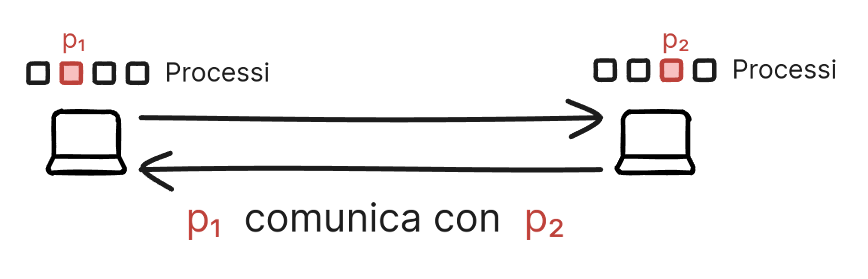
\includegraphics[width=0.7\textwidth]{comunicazione-processi}
  \caption{Comunicazione tra processi}
\end{figure}
Un flusso di comunicazione è identificato univocamente dalla tupla:
\[
  (IP_A, IP_B, Porta_A, Porta_B)
\]
La porta viene assegnata ad un processo soltanto quando esso inizia a comunicare.

\subsubsection{Ottenimento dell'IP e della porta}
Queste informazioni sono contenute negli header aggiunti ad ogni livello.
\begin{figure}[H]
  \centering
  \begin{tikzpicture}
    \node[draw, minimum width=5cm, minimum height=1cm] at (0.45,0) (m) {Messaggio};
    \draw[->] (m.south) -- ++(0,-1);

    \coordinate (a) at (-2.7,-3);
    \draw (a) rectangle ++(1,1) node[midway] {$m_1$};
    \draw[blue,fill, fill opacity=0.1] (a) ++(0,1) rectangle ++(-0.5,-1);

    \coordinate (b) at (-0.8,-3);
    \draw (b) rectangle ++(1,1) node[midway] {$m_2$};
    \draw[blue,fill, fill opacity=0.1] (b) ++(0,1) rectangle ++(-0.5,-1);

    \coordinate (c) at (1.1,-3);
    \draw (c) rectangle ++(1,1) node[midway] {$m_3$};
    \draw[blue,fill, fill opacity=0.1] (c) ++(0,1) rectangle ++(-0.5,-1);

    \coordinate (d) at (2.9,-3);
    \draw (d) rectangle ++(1,1) node[midway] {$m_4$};
    \draw[blue,fill, fill opacity=0.1] (d) ++(0,1) rectangle ++(-0.5,-1);
    \draw[<-,blue] (d) ++(-0.25,1) -- ++(0,0.5) node[above,blue] {Porta};
    \draw[blue] (d) ++(1.25,0.5) node[right,align=center] {Livello\\trasporto};

    \draw[->] (m.south) ++(0,-3) -- ++(0,-1);

    \coordinate (e) at (-3.7,-6);
    \draw (e) rectangle ++(1,1) node[midway] {$m_1$};
    \draw[blue,fill, fill opacity=0.1] (e) ++(0,1) rectangle ++(-0.5,-1);
    \draw[red,fill, fill opacity=0.1] (e) ++(-0.5,1) rectangle ++(-0.5,-1);

    \coordinate (f) at (-1.3,-6);
    \draw (f) rectangle ++(1,1) node[midway] {$m_2$};
    \draw[blue,fill, fill opacity=0.1] (f) ++(0,1) rectangle ++(-0.5,-1);
    \draw[red,fill, fill opacity=0.1] (f) ++(-0.5,1) rectangle ++(-0.5,-1);

    \coordinate (g) at (1.1,-6);
    \draw (g) rectangle ++(1,1) node[midway] {$m_3$};
    \draw[blue,fill, fill opacity=0.1] (g) ++(0,1) rectangle ++(-0.5,-1);
    \draw[red,fill, fill opacity=0.1] (g) ++(-0.5,1) rectangle ++(-0.5,-1);

    \coordinate (h) at (3.5,-6);
    \draw (h) rectangle ++(1,1) node[midway] {$m_4$};
    \draw[blue,fill, fill opacity=0.1] (h) ++(0,1) rectangle ++(-0.5,-1);
    \draw[red,fill, fill opacity=0.1] (h) ++(-0.5,1) rectangle ++(-0.5,-1);
    \draw[<-,red] (h) ++(-0.75,1) -- ++(0,0.5) node[above,red] {IP};
    \draw[red] (h) ++(1.25,0.5) node[right,align=center] {Livello\\di rete};

  \end{tikzpicture}
  \caption{Porta e IP}
\end{figure}

\noindent
Un pacchetto si può rappresentare nel seguente modo:
\begin{figure}[H]
  \centering
  \begin{tikzpicture}
    \draw[red] (0,0) rectangle ++(1,1);
    \node[red,above,scale=0.8,align=center] at (0.5,1) {Header\\livello\\di rete};

    \draw[dashed,blue] (0,0) ++(1.1,0.1) rectangle ++(0.8,0.8);
    \draw (0,0) ++(1,0) rectangle ++(4,1);

    \draw (0,0) ++(1,-0.2) -- ++(0,-0.2) -- ++(4,0) node[midway,below] {Payload}
      -- ++(0,0.2);
  \end{tikzpicture}
  \caption{Rappresentazione di un pacchetto}
\end{figure}
\noindent
oppure si può rappresentare anche come:
\begin{figure}[H]
  \centering
  \begin{tikzpicture}
    \draw[red] (0,0) rectangle ++(3,2) node[midway,above,align=center,scale=0.85,yshift=-0.5cm] {
        \texttt{01011100101101001}\\
        \texttt{01010011101101001}\\
        \texttt{10010110011010101}\\
      };
    \node[draw,red,scale=0.8,minimum width=3.5cm] at (1.5,0.3) {IP Destinazione};
    \node[draw,red,scale=0.8,minimum width=3.5cm] at (1.5,0.75) {IP Sorgente};

    \draw (0,0) rectangle ++(3,-3) node[midway,align=center,scale=0.9] 
      {
       \texttt{01011100101101001}\\
       \texttt{01010011101101001}\\
       \texttt{10010110011010101}\\
       \texttt{10101010110111010}\\
       \texttt{11101010100101000}\\
       \texttt{01010001110010110}\\
       \texttt{11101010110101100}
     };

   \draw[red] (3.1,0.1) -- ++(0.2,0) -- ++(0,0.85) node[midway,right,align=left] 
     {Dati sempre\\presenti} -- ++(-0.2,0);
  \end{tikzpicture}
\end{figure}

\section{Indirizzi IP}
Sono identificativi \textbf{univoci} di un'interfaccia di un host della rete Internet.
Un end system può avere soltanto un'interfaccia, ma un router deve avere minimo 2
interfacce per poter permettere la comunicazione tra più entità.


\begin{example}
  Un esempio di indirizzo IP è:
  \[
    1001 \; 1101 \;\; 0001 \; 1011 \;\; 0001 \; 0011 \;\; 0111 \; 1011
  \] 
  Per facilitare la lettura e la gestione degli indirizzi IP si usa la notazione
  \textbf{decimale puntata}. In questa notazione si considerano blocchi di 8 bit, di
  conseguenza si avranno 4 blocchi. Ogni blocco viene tradotto in un numero intero decimale
  compreso tra 0 e 255 e separato da un punto:
  \[
    157.27.19.123
  \] 
\end{example}

\subsection{Suddivisione dei bit}
I bit dell'indirizzo IP hanno tutti la stessa importanza?

\vspace{1em}
\noindent
Prendiamo ad esempio i numeri telefonici della rete fissa:
\[
  \underbrace{0039 \; 045 \; 802}_{\text{Prefisso}} \; \underbrace{7059}_{\text{Suffisso}}
\] 
\begin{itemize}
  \item Il prefisso è l'identificativo di una specifica organizzazione
  \item Il suffisso identifica un utente specifico all'interno dell'organizzazione
\end{itemize}

\vspace{1em}
\noindent
Allo stesso modo in un indirizzo IP si ha \textbf{prefisso} e \textbf{suffisso}
\begin{itemize}
  \item \textbf{Prefisso}: Identifica una rete specifica
  \item \textbf{Suffisso}: Identifica un'interfaccia di un host di una specifica rete 
\end{itemize}

\subsubsection{Identificazione del prefisso e del suffisso}
Nel caso dei numeri telefonici si inserisce una barra per separare il prefisso dal suffisso:
\[
  045/7021412
\]
Negli indirizzi IP il numero di bit dedicati al prefisso dipende dalla dimensione della
rete ed è indicato da una barra seguita da un numero.
\[
  157.27.19.123/16
\] 
Significa che i primi 16 bit dell'indirizzo IP sono dedicati al prefisso.
\[
  \underbrace{10011101 \;\; 00011011}_{n} \;\; \underbrace{00010011 \;\; 01111011}_{32 - n}
\] 
Quindi il numero di indirizzi si calcola come:
\[
  \text{indirizzi} = 2^{32-n}
\] 
\begin{example}
  \[
    n = 20 \to 2^{12} = 4096
  \] 
  \[
    n = 24 \to 2^8 = 256
  \] 
\end{example}

\noindent
Per identificare il numero di bit del prefisso i calcolatori utilizzano una sequenza di
32 bit in cui i bit associati al prefisso sono posti a \( 1 \) e gli altri a \( 0 \),
ad esempio:
\[
/16 \to 11111111 \;\; 11111111 \;\; 00000000 \;\; 00000000
\] 
Questa sequqnza è chiamata \textbf{maschera} perchè è abbinata all'indirizzo IP.
\begin{example}
\[
  \begin{aligned}
    \text{IP: } & \,10011101 \;\; 00011011 \;\;\, 00010011 \;\; 01111011\\
    \text{Mask: }& \underbrace{11111111 \;\; 11111111}_{\text{Prefisso}} \;\; \underbrace{00000000 \;\; 00000000}_{\text{Suffisso}}
  \end{aligned}
\] 
\end{example}
Facendo l'AND bit a bit tra l'IP e la maschera si ottiene l'indirizzo di rete a cui
quell'indirizzo IP appartiene.

\vspace{1em}
\noindent
La maschera può essere rappresentata anche in:
\begin{itemize}
  \item \textbf{Notazione decimale puntata}:
    \[
      /16 \to 255.255.0.0
    \] 
  \item \textbf{Notazione esadecimale}: si divide l'IP in gruppi da 4 bit e si convertono
    in esadecimale:
    \[
      /16 \to \texttt{0xffff0000}
    \] 
    Per capire che un numero è esadecimale, esso è prefissato da \texttt{0x}.
\end{itemize}

\subsection{Indirizzi IP riservati}
Non tutti gli indirizzi IP possono essere assegnati a degli host, infatti ce ne sono alcuni
riservati per delle funzioni specifiche:
\begin{enumerate}
  \item \textbf{This host}: È l'indirizzo IP del calcolatore stesso
    \[
      0.0.0.0
    \] 
  \item \textbf{Local broadcast} (o limited broadcast): Indirizzo IP che permette di 
    inviare un messaggio a tutti i calcolatori della rete locale
    \[
      255.255.255.255
    \]
  \item \textbf{Indirizzo di rete}: I primi \( n \) bit identificano una rete, gli altri
    \( 32 - n \) sono tutti posti a 0. Questo IP identifica la rete e nessun host può
    avere questo indirizzo
    \[
      \underbrace{1010100011}_{n} \underbrace{0000000000000000000000}_{32-n}
    \] 
  \item \textbf{Directed broadcast}: È un IP che permette di mandare un messaggio a tutti
    gli utenti di una rete specifica, anche esterna alla rete locale
    \[
      \underbrace{1010100011}_{n} \underbrace{1111111111111111111111}_{32-n}
    \] 
\end{enumerate}

\subsection{Conoscere il proprio indirizzo IP}
L'indirizzo ip e la dimensione del prefisso dipendono dalla rete a cui si è collegati.
Per conoscere il proprio indirizzo ip si usa il comando: \texttt{ifconfig}
\begin{figure}[H]
  \centering
  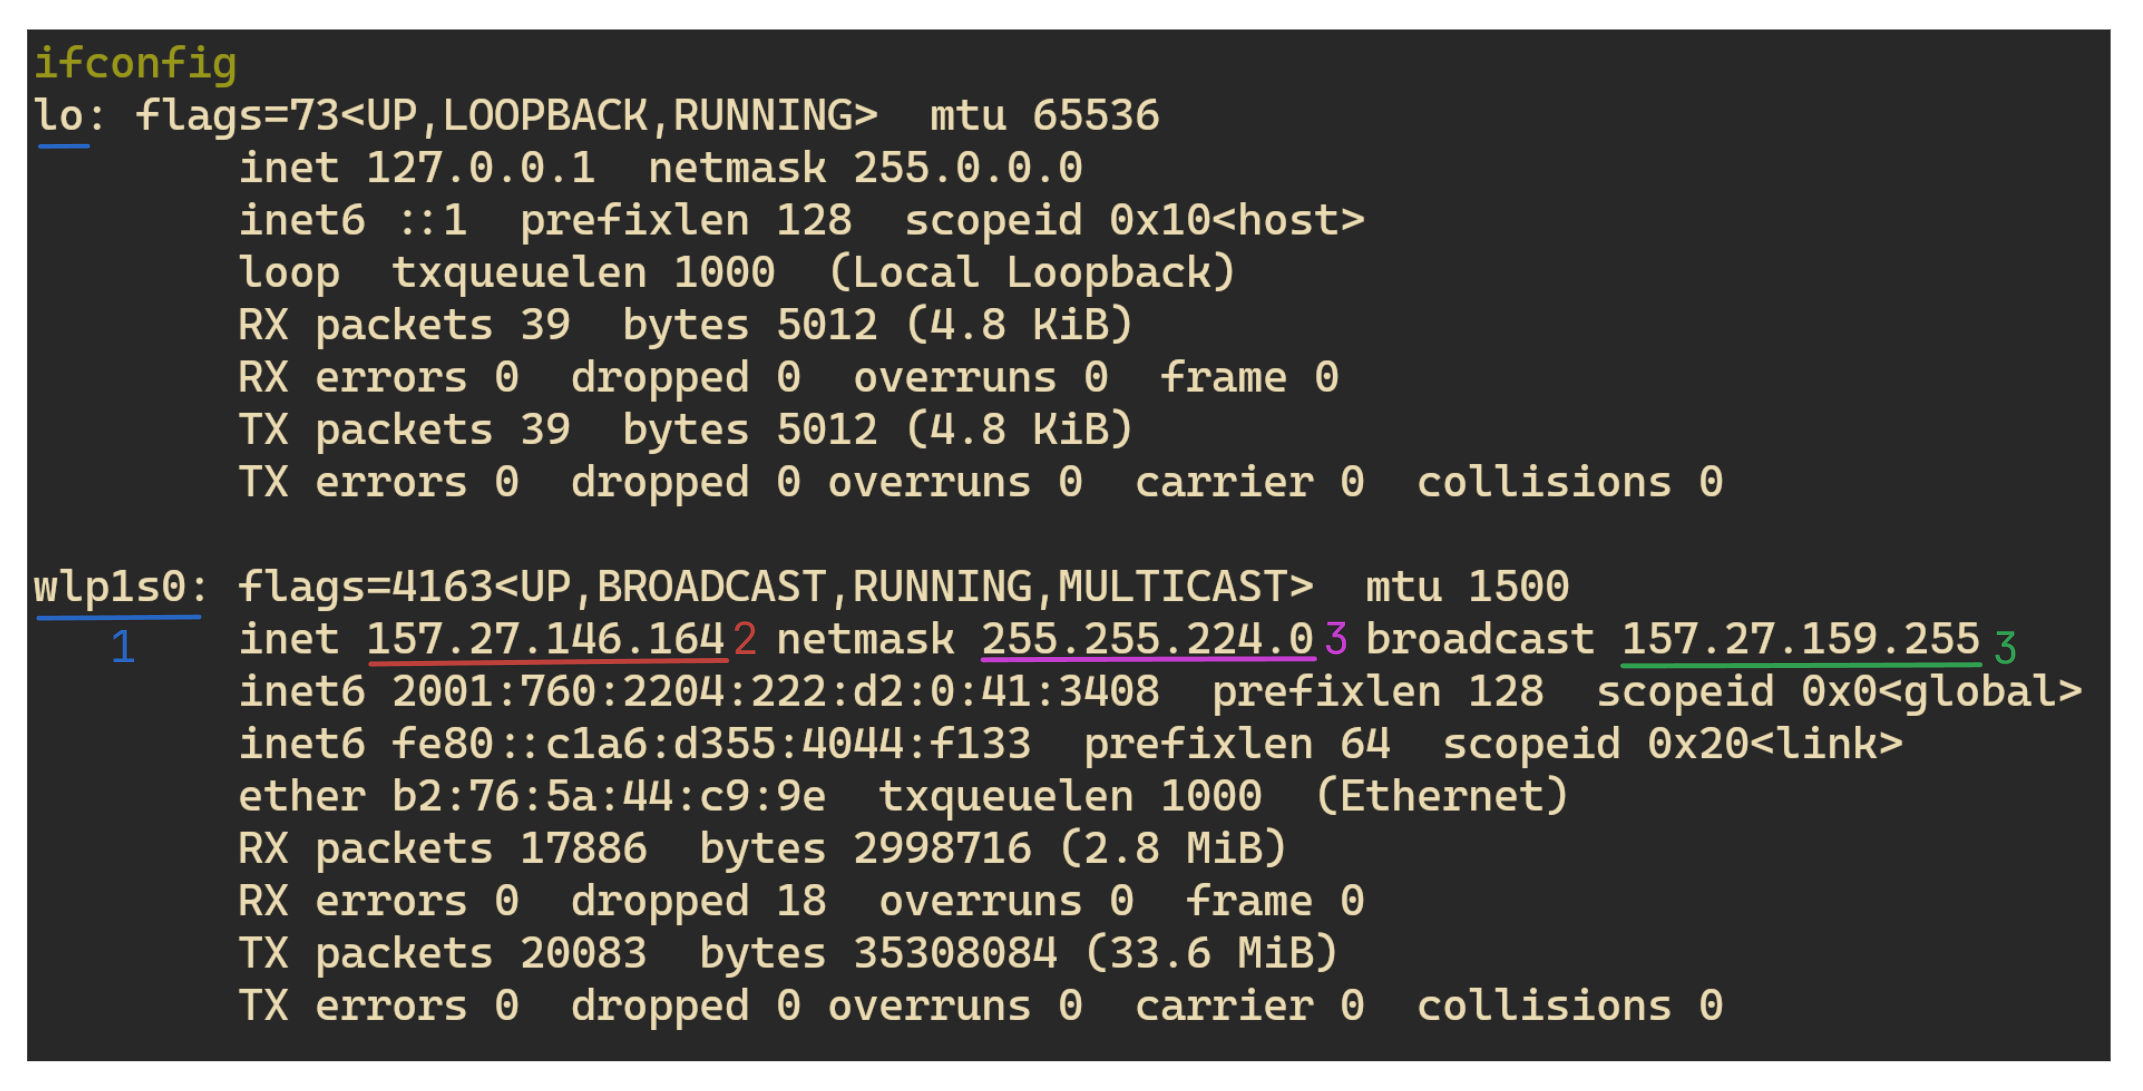
\includegraphics[width=1\textwidth]{ifconfig}
\end{figure}
\begin{enumerate}
  \item \textbf{Interfaccia di rete}: Rappresenta il collegamento tra il calcolatore e
    la rete.
  \item \textbf{Indirizzo ip}
  \item \textbf{Indirizzo broadcast}
  \item \textbf{Maschera}
\end{enumerate}

\vspace{1em}
\noindent
Altre informazioni sulla rete si possono ottenere con il comando: \texttt{whois}.
Questo comando si connette ad un server che contiene informazioni sugli indirizzi IP.

\noindent
L'output di questo comando da varie informazioni sull'IP messo come argomento, ma si
può notare che la maschera è diversa da quella che viene data in output dal comando
\texttt{ifconfig}.

\begin{itemize}
  \item Per \texttt{ifconfig} il prefisso è da 20 bit, quindi \( 2^{12} = 4096 \) indirizzi
  \item per \texttt{whois} il prefisso è da 16 bit, quindi \( 2^{16} = 65536 \) indirizzi
\end{itemize}

\noindent
Questo è dovuto al \textbf{subnetting}, cioè la creazione di sottoreti per partizionare
l'organizzazione distribuita sul territorio, quindi dei \( 65546 \) indirizzi, alcuni
verranno assegnati ad una sottorete e altri ad un'altra.
\begin{figure}[H]
  \centering
  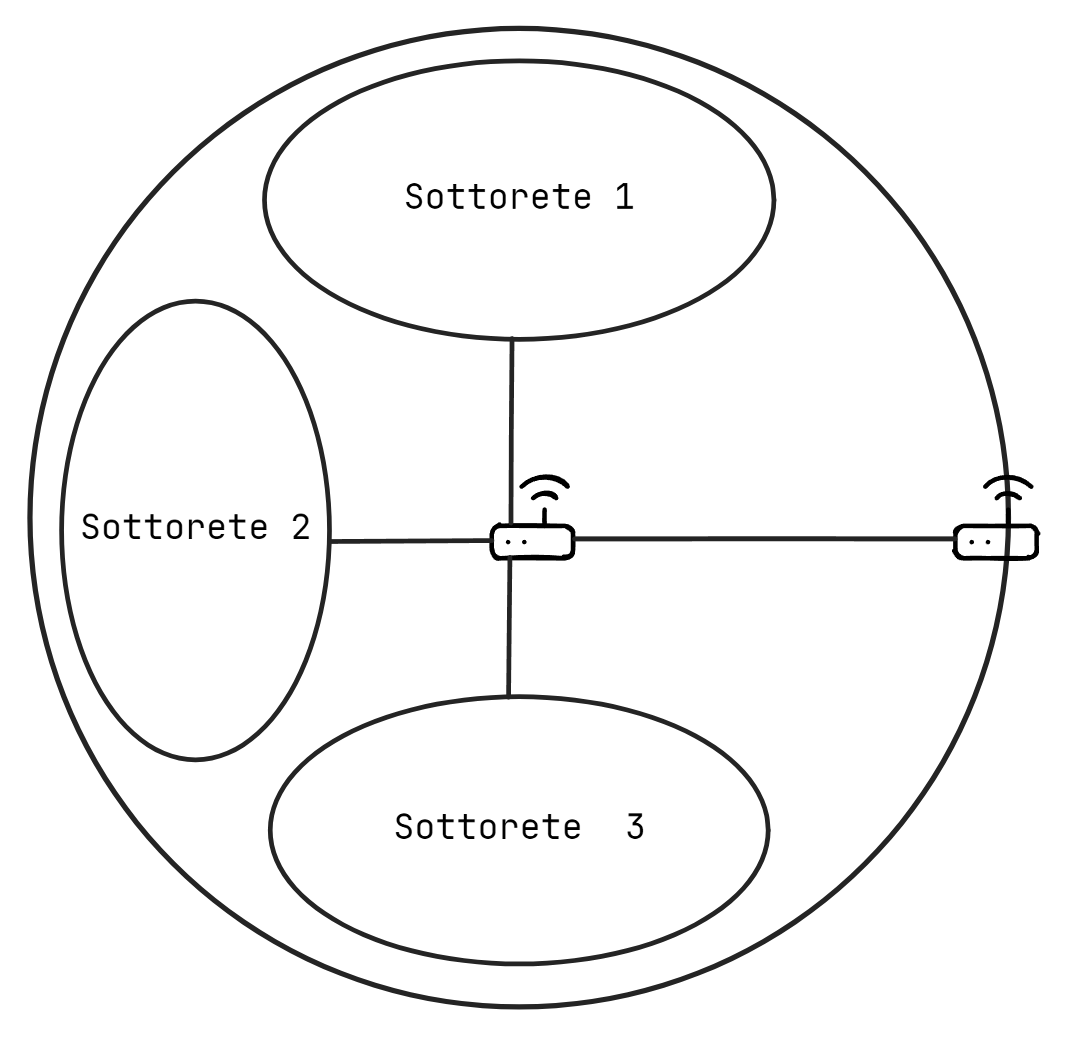
\includegraphics[width=0.70\textwidth]{subnetting}
  \caption{Subnetting}
\end{figure}
\noindent
Questa suddivisione dall'esterno non viene vista e questo è il motivo per cui ipconfig
mostra una maschera diversa da quella che si vede con il comando \texttt{whois}.

\subsection{Esercizi}
Conversione di IP decimale/binario
\begin{exercise}
  Dato il seguente IP:
  \[
    1110 \; 0111 \;\; 1101 \; 1011 \;\; 1000 \; 1011 \;\; 0110 \; 1111
  \] 
  la traduzione in decimale è la seguente:
  \[
    231.219.139.111
  \] 
\end{exercise}
\begin{exercise}
  Dato il seguente IP:
  \[
    221.34.255.82
  \] 
  la traduzione in binatio è la seguente:
  \[
    1101 \; 1101 \;\; 0010 \; 0010 \;\; 1111 \; 1111 \;\; 0101 \; 0010
  \] 
\end{exercise}

\subsection{Subnetting}
È il processo che permette di suddividere una rete in sottoreti.

\subsubsection{Creazione delle sottoreti partendo da un blocco di indirizzi assegnato}
Un'organizzazione richiede un blocco di indirizzi in base alle proprie necessità.
Prendendo come esempio l'Università di Verona, essa ha come indirizzo di rete il seguente:
\[
  157.27.0.0/16
\] 
si nota che i primi 16 bit sono dedicati al prefisso:
\[
  \underbrace{10011101 \;\; 00011011}_{\text{Prefisso}} \;\; \underbrace{00000000 \;\; 00000000}_{\text{Suffisso}}
\] 
Partendo da tale blocco si vogliono creare 2 sottoreti di pari dimensione. Per fare ciò
si può prendere il primo bit del suffisso, separarlo dal suffisso e associarlo al prefisso.
\[
  \underbrace{10011101 \;\; 00011011}_{\text{Prefisso}} \;\;
  \underbrace{0}_{\text{Sottorete}} \;\;
  \underbrace{0000000 \;\; 00000000}_{\text{Suffisso}}
\] 
Il bit assegnato al prefisso può avere 2 valori, quindi si possono creare 2 sottoreti:
\[
  \begin{aligned}
    \text{Sottorete 1: } &
    \underbrace{10011101 \;\; 00011011 \;\;\; 0}_{\text{Prefisso}} \;\;
    \underbrace{0000000 \;\; 00000000}_{\text{Suffisso}}\\
    \text{Sottorete 2: } &
    \underbrace{10011101 \;\; 00011011 \;\;\; 1}_{\text{Prefisso}} \;\;
    \underbrace{0000000 \;\; 00000000}_{\text{Suffisso}}
  \end{aligned}
\]
In notazione decimale puntata diventa:
\[
  \begin{aligned}
    \text{Sottorete 1: } &
    157.27.0.0/17\\
    \text{Sottorete 2: } &
    157.27.128.0/17
  \end{aligned}
\]
Quello che cambia è che il prefisso è diventato di 17 bit.

\vspace{1em}
\noindent
Da un blocco \( /16 \to 2^{32-16} = 65536 \) indirizzi si ottengono 2 blocchi
\( /17 \to 2^{32-17} = 2^{15} = 32768 \) indirizzi ciascuno.
\begin{figure}[H]
  \centering
  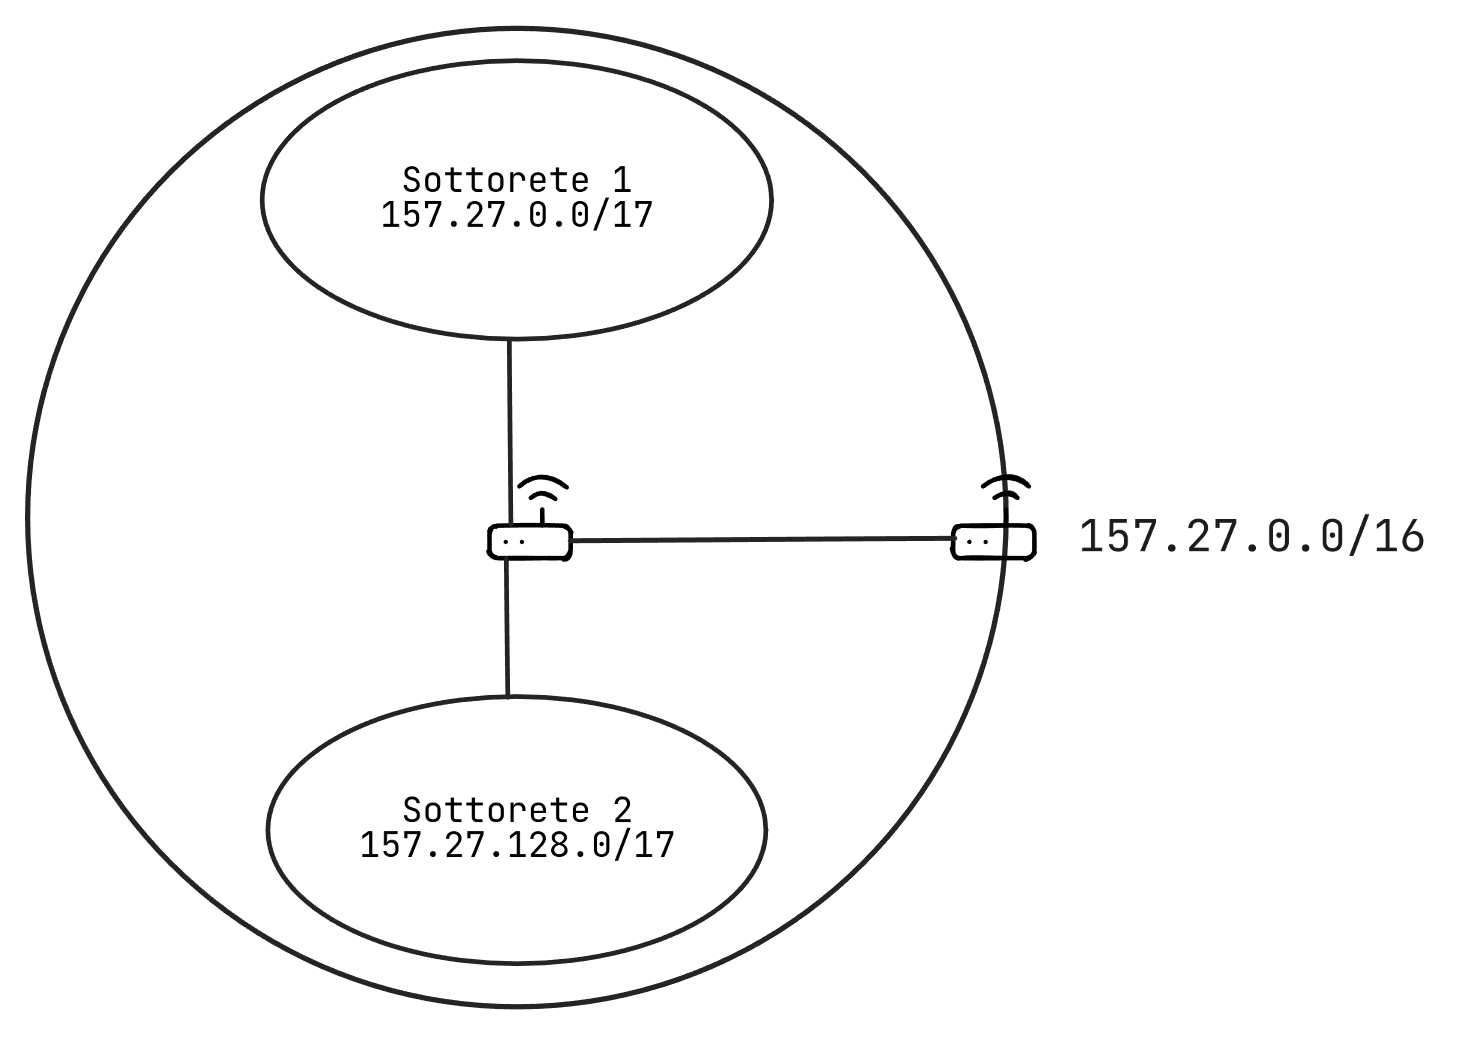
\includegraphics[width=0.70\textwidth]{esempio-subnetting}
  \caption{Risultato del subnetting}
\end{figure}

\noindent
I blocchi di indirizzi si chiamano \textbf{CIDR} (Classless Inter-Domain Routing).

\begin{itemize}
  \item \textbf{Nota storica}: In passato si usava la notazione \textbf{classful} in cui
    il numero di bit dedicati al prefisso era predererminato e venivano usati i bit
    iniziali per distinguere i diversi casi. Ad esempio:
    \begin{itemize}
      \item \textbf{Classe A}: 8 bit di prefisso se l'IP iniziava con 0:
        \[
          \underbrace{0 \;\;\; 1010010}_{\text{Prefisso}} \;\; \underbrace{00000000 \;\; 00000000 \;\; 00000000}_{\text{Suffisso}}
        \] 
      \item \textbf{Classe B}: 16 bit di prefisso se l'IP iniziava con 10:
        \[
          \underbrace{10 \;\;\; 010010 \;\; 10110100}_{\text{Prefisso}} \;\; \underbrace{00000000 \;\; 00000000}_{\text{Suffisso}}
        \]
      \item \textbf{Classe C}: 24 bit di prefisso se l'IP iniziava con 110:
        \[
          \underbrace{110 \;\;\; 010010 \;\; 10110100 \;\; 00000000}_{\text{Prefisso}} \;\; \underbrace{00000000}_{\text{Suffisso}}
        \]
    \end{itemize}
    L'informazione del prefisso era codificata nell'indirizzo stesso e quindi non c'era
    bisogno di aggiungere un'informazione all'IP come ad esempio la maschera.

    Per l'alta richiesta di indirizzi, l'indirizzamento classful non era sufficiente:
    \begin{table}[H]
      \centering
      \begin{tabular}{c|c|c}
        Classe & N° reti              & N° host              \\
        \hline
             A & $2^{7} \approx 16K$  & $2^{24} \approx 16M$ \\
             B & $2^{14} \approx 16K$ & $2^{16} \approx 65K$ \\
             C & $2^{21} \approx 2M$  & $2^{8} \approx 256$  \\
      \end{tabular}
    \end{table}
    \noindent
    Si esaurirono presto le classi A e B, quindi si passò al CIDR.
\end{itemize}

\vspace{1em}
\noindent
A volte assegnare delle sottoreti di uguale dimensione è uno spreco perchè certe esigenze
richiedono meno indirizzi e altre di più, quindi si dovrebbe suddividere la rete in sottoreti 
di dimensione \textbf{diversa}.

\section{Livello applicativo}
Il livello applicativo è il livello più alto dello stack protocollare:
\begin{figure}[H]
  \centering
  \begin{tikzpicture}[scale=0.8]
    \draw[fill,blue,fill opacity=0.2,text=black,text opacity=1] (0,4) rectangle ++(3,1) node[midway] {Applicazione};
    \draw (0,3) rectangle ++(3,1) node[midway] {Trasporto};
    \draw (0,2) rectangle ++(3,1) node[midway] {Rete};
    \draw (0,1) rectangle ++(3,1) node[midway,align=center] {Collegamento\\dati};
    \draw (0,0) rectangle ++(3,1) node[midway] {Fisico};
  \end{tikzpicture}
  \caption{Stack TCP/IP}
\end{figure}

\noindent
Questo livello genera un messaggio che può essere di tipo diverso, ad esempio:
\begin{itemize}
  \item Richiesta HTTP
  \item Risposta HTTP
  \item Email
  \item Il frame di un video
\end{itemize}
Quando un messaggio viene generato da un'applicazione si deve decidere quale protocollo
utilizzare a livello di trasporto:
\begin{itemize}
  \item \textbf{TCP} (Transmission Control Protocol): È un protocollo orientato
    alla connessione (\textbf{Connection oriented}) e affidabile. Questo protocollo da
    la garanzia che il messaggio arrivi a destinazione.
  \item \textbf{UDP} (User Datagram Protocol): È un protocollo non orientato alla
    connessione (\textbf{Connectionless}) e non affidabile. Questo protocollo non da la
    garanzia che il messaggio arrivi a destinazione e quindi non è detto che il messaggio
    arrivi.
\end{itemize}

\noindent
Un servizio di trasporto \textbf{affidabile} garantisce che la consegna arrivi a destinazione.

\subsection{Esempi di applicazioni e relativi protocolli di trasporto}
\begin{itemize}
  \item \textbf{Web}:
  Un esempio di applicazione è il browser web che utilizza il protocollo \texttt{HTTP}
  per trasferire dati attraverso la rete. Quando si consegnano testo e immagini
  non si devono commettere errori, quindi in questi casi il protocollo \texttt{HTTP}
  si appoggia a TCP.

  \item \textbf{Posta elettronica}:
  Un'altro esempio è la posta elettronica che utilizza il protocollo \texttt{SMTP}
  per inviare la posta. Questo protocollo richiede un servizio affidabile, quindi
  se un pacchetto viene perso, il protocollo TCP si preoccupa di recuperarlo.

  \item \textbf{Audio/video}:
  Per la trasmissione di audio e video di solito i protocolli sono proprietari, ma in
  questo caso non è necessaria l'affidabilità, basta garantire la tolleranza alle
  perdite, quindi ci si appoggia al protocollo UDP.

  \item \textbf{DNS}:
  Per navigare su internet si usa il protocollo \textbf{DNS} (Domain Name System)
  che è il servizio che traduce i nomi logici nei corrispettivi indirizzi ip.
\end{itemize}

\subsection{Socket}
Quando un'applicazione deve mandare un messaggio ad un'altra applicazione essa apre
un \textbf{socket} verso la destinazione. Un socket è un'interfaccia di comunicazione 
(astrazione software) che identifica un flusso informativo bidirezionale. Per aprire un
socket bisogna specificare:
\begin{itemize}
  \item Protocollo di trasporto
  \item Indirizzo IP di destinazione
  \item Indirizzo IP sorgente
  \item Porta di destinazione
  \item Porta di sorgente
\end{itemize}
L'apertura di un socket è effettuata soltanto da uno dei due processi.
\begin{figure}[H]
  \centering
  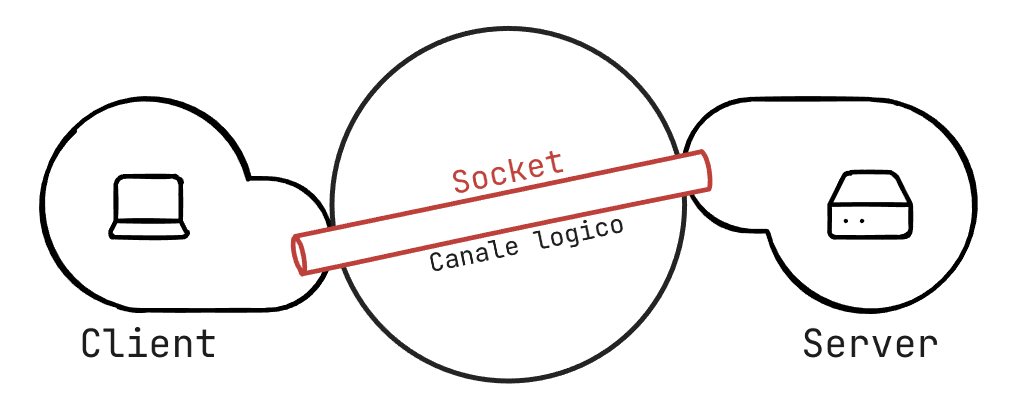
\includegraphics[width=0.7\textwidth]{socket}
\end{figure}

\noindent
Tra i due processi comunicanti si possono identificare due ruoli distinti:
\begin{enumerate}
  \item \textbf{Processo Client}: È il processo che è responsabile dell'inizio della
    comunicazione. Il client ha un indirizzo IP dinamico, cioè cambia in base alla
    rete a cui è collegato.

  \item \textbf{Processo Server}: È il processo che sta su un host sempre raggiungibile
    e sempre in ascolto. Il server ha un indirizzo IP statico.
\end{enumerate}

\subsection{Protocolli}
\subsubsection{Protocollo HTTP}
Il protocollo \textbf{HTTP} (HyperText Transfer Protocol) è un protocollo di livello
applicativo usato per la trasmissione di documenti ipertestuali. Questo protocollo
è di tipo \textbf{testuale} (i messaggi sono scritti in ASCII),
determina il formato dei messaggi ed è basato sul modello \textbf{richiesta/risposta}:
\begin{itemize}
  \item \textbf{Richiesta}: Il client apre un socket, invia un messaggio di richiesta
    al server e aspetta la risposta.
  \item \textbf{Risposta}: Il server deve inviare un messaggio di risposta alla richiesta 
    del client
\end{itemize}
Se la richiesta non fosse ben formata il server risponde con un messaggio di errore.
Per cui il protocollo prevede sempre, ad ogni richiesta, che ci sia una risposta, positiva
o negativa.

Il server contiene delle pagine web, con eventualmente altri contenuti ad esempio immagini.
Il file di testo principale (\texttt{index.html}).
\begin{figure}[H]
  \centering
  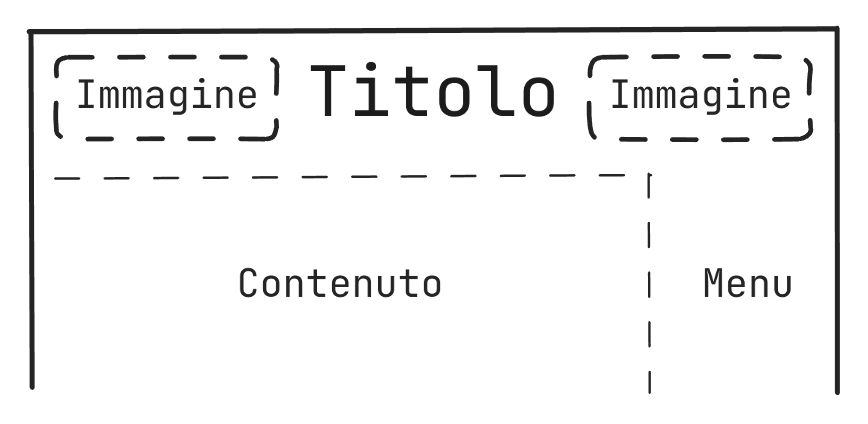
\includegraphics[width=0.7\textwidth]{html}
\end{figure}
\noindent
Un file \texttt{html} definisce sia la struttura che il contenuto di una pagina web.
\begin{figure}[H]
  \centering
  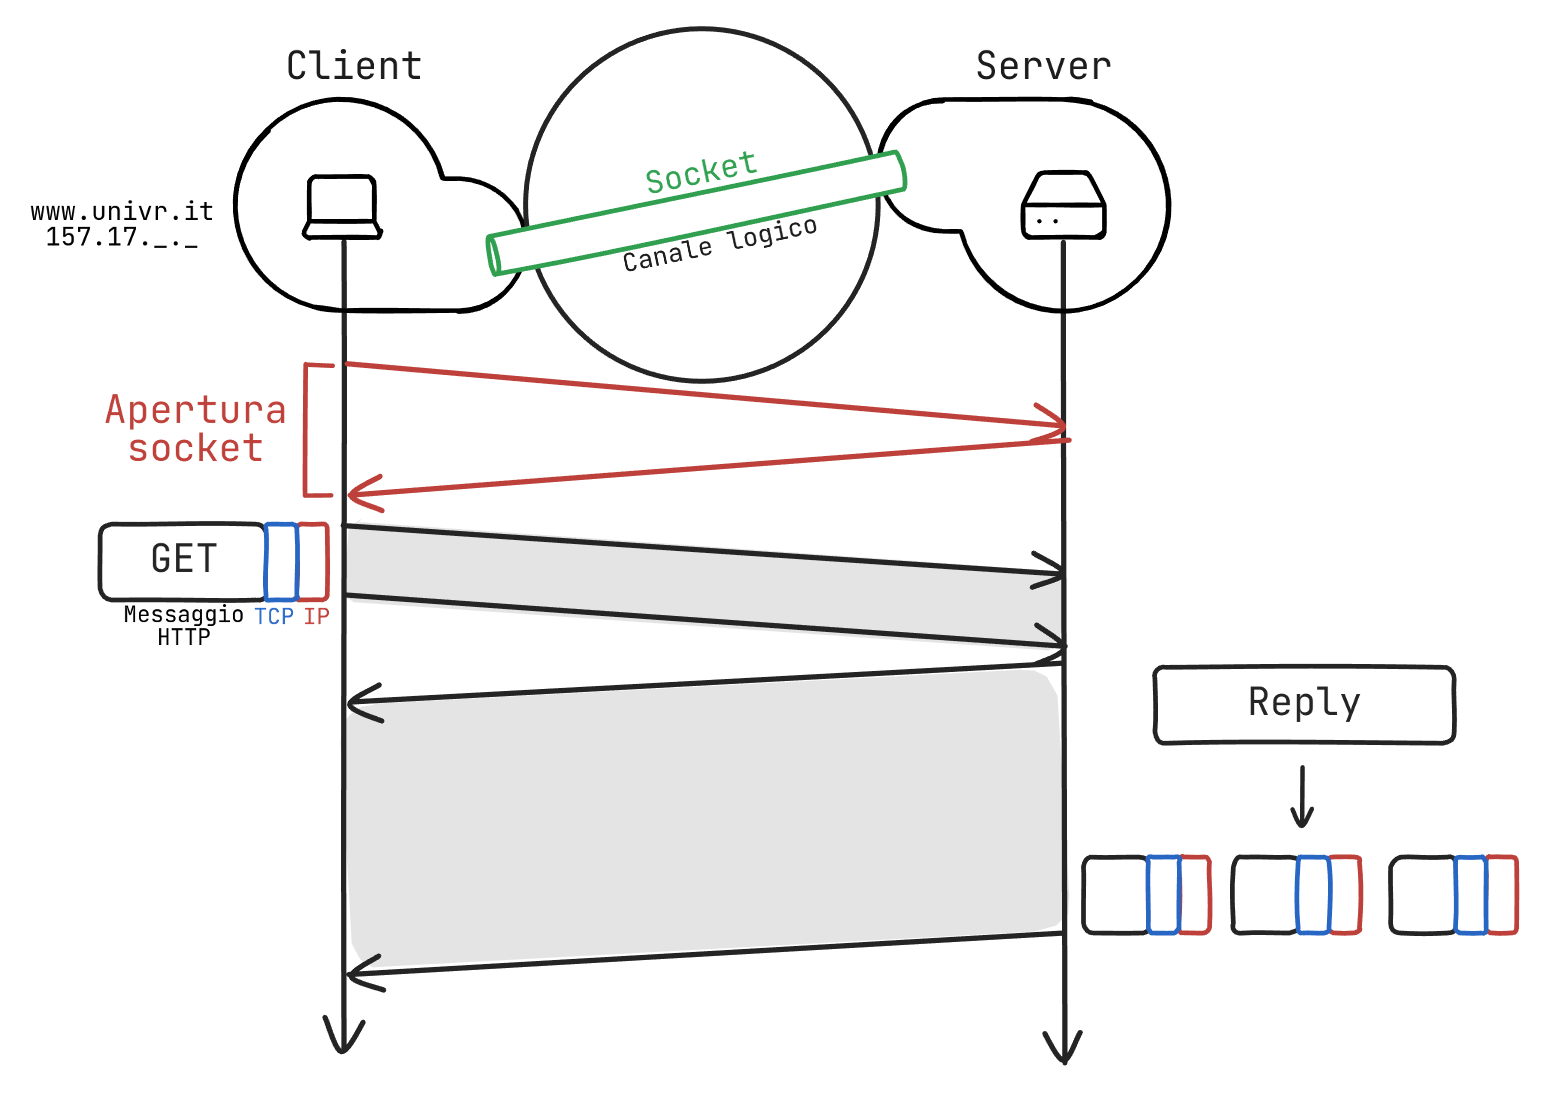
\includegraphics[width=0.9\textwidth]{comunicazione-socket}
\end{figure}

\vspace{1em}
\noindent
La struttura dei messaggi HTTP è la seguente:
\begin{enumerate}
  \item Riga di richiesta
  \item Una o più righe di intestazione
\end{enumerate}

\begin{example}
  Un'esempio di richiesta HTTP è:
  \begin{lstlisting}[language=Scala, title=sas]
    GET /index.html HTTP/1.1 // -- Riga di richiesta
    Host: www.univr.it       // -+ Righe di
    User-Agent: Mozilla/5.0  // -+ intestazione
    Accept-language: en      // (facoltativo)
  \end{lstlisting}
  che corrisponde a una richiesta di una pagina web del seguente tipo:
  \[
    \underbrace{\texttt{www.univr.it}}_{\text{Server}} 
      \underbrace{\texttt{/index.html}}_{\text{File richiesto}}
  \]
\end{example}

\end{document}
